%\section{Identifying Devices by Features}
\section{Disaggregation Features}
\label{sec:features}
%Previous surveys have summarized the features for energy disaggregation, primarily from an
%electrical engineering viewpoint [\citeNP{zeifman2011nonintrusive,lee2004exploration,
%liang2010load,zoha2012survey}].
%We target this survey for the data mining community and complement prior literature 
%by providing details of existing features and newer ones, and 
%summarizing the strengths and weaknesses of these features in disaggregation.
%and add the computational cost of each approach. 
%

%\manishc{like we discussed, focus this section on features, and move data
%  collection to later}
%\huijuanc{ok. already moved.}
In this section we briefly outline several features that are used in disaggregation and
classify them based on different types like AC vs. non-AC or steady vs. transient state. 
%Data collection methods and instrumentation used 
%We also present techniques and methodologies by which the data is collected to assist feature
%extraction for the learning algorithms. 
%%\section{Experiments Setup and Data Sets}
\subsection{Data Collection  and Public Data Sets}
\label{sec:setup}
The usefulness of energy disaggregation algorithms is a function of the aggregated datasets' 
availability. 
Therefore we need to collect this data by installing the corresponding meters and 
sensors and setting up the necessary experiments. 

\subsubsection{Meters}
Generally speaking,
there are two types of data that can be used to disaggregate devices:
AC power information and non-AC power information.
To obtain AC power data, a real power meter, reactive power meter,
ammeter, and voltage meter (usually consolidated into one meter) can be installed to
record different power values, current or voltage values, 
and noise generated by power line.  
Sensors are installed to collect non-AC power data, like electromagnetic fields (EMF) 
around devices~\cite{giri_study_2012}, light, and sound~\cite{kim2009viridiscope}.

Figure~\ref{fig_metersConnection} illustrates how
four types of meters/sensors are installed in a building.
After two-phase power is delivered into the home, %\manishc{usually homes have 2-phase},
three power meters, which record real power,
current, and voltage are installed on
these three entry power lines separately. 
A power meter is installed on each circuit, such as for the refrigerator,
 to monitor the
true status of the devices (to validate results).
A sensor is plugged into the outlet to monitor the
voltage noise data.
Besides these AC-power meters,
an electromagnetic field sensor, 
a sound sensor , and a light sensor
may also be installed around devices,
such as the refrigerator, to capture its electrical magnetic field, 
sound-related, and light-related operations.

\begin{figure}[ht]
\centering
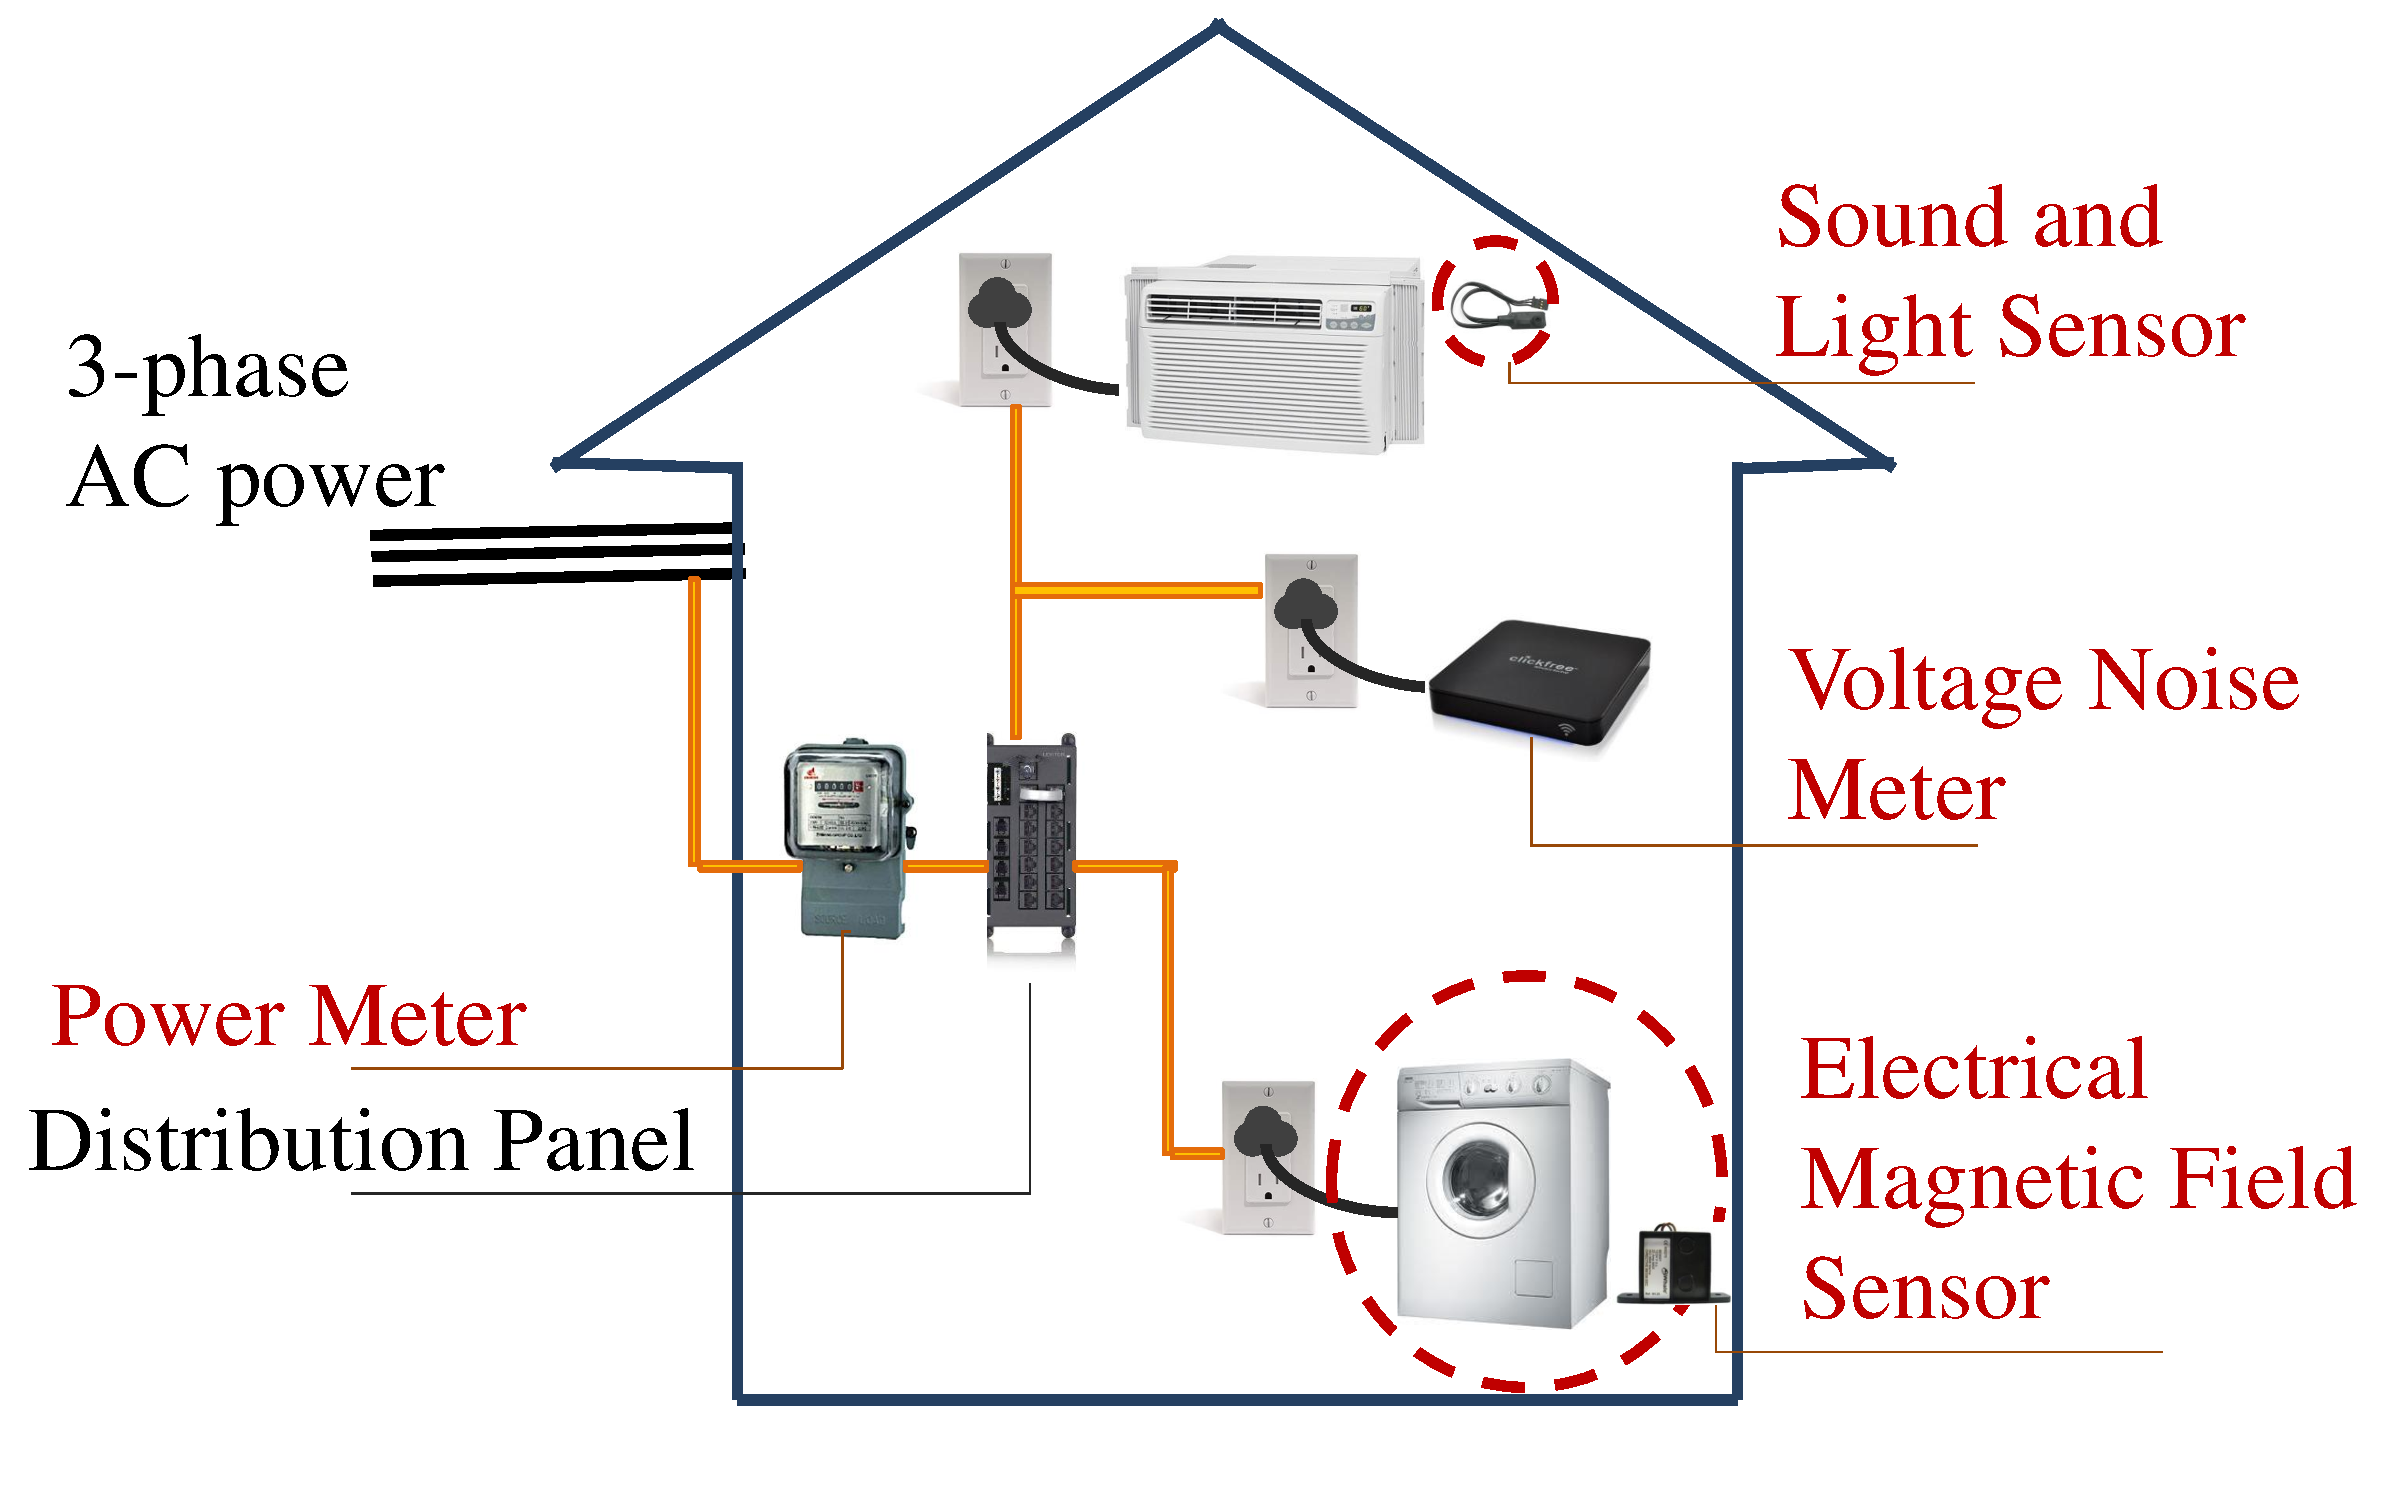
\includegraphics[width=3 in]{figs/metersConnection.pdf}
\caption{Four Types of Meters in a Building.}
\label{fig_metersConnection}
\end{figure}

\begin{table}
\caption{Meters Used in Experiments.}
\small
\label{tab_meters}
\begin{center}
\makebox{
\begin{tabular} {|l|l|l|l|}
\hline
Meter Types & Meter Name & Meter Example & Recorded Features \\
\hline
\multirow{4}{*}{AC power} & ammeter & TED, LEM LA55-P~\cite{meterTED} & AC waveform, harmonics \\
\cline{2-4}
& voltage meter & Pico TA041~\cite{meterPico}& voltage waveform, voltage \\
\cline{2-4}
& real power meter & National Instruments USB-9215A~\cite{meterNI} & real power \\
\cline{2-4}
& reactive power meter & TrendPoints EnerSure~\cite{meterTrend}& reactive power \\
\cline{2-4}
& voltage noise meter & Build by author & voltage noise \\
\hline
\multirow{3}{*}{Non-AC power} & electromagnetic field meter & Trifield~\cite{meterEMF}&electromagnetic field \\
\cline{2-4}
& sound sensor& mindstorms~\cite{meterSound}& sound strongness \\
\cline{2-4}
& light sensor & extech~\cite{meterLight}& light strongness \\
\cline{2-4}
& temperature meter & amprobe~\cite{meterTemp}& temperature\\
\hline
\end{tabular}}
\end{center}
\end{table}


The meters or sensors that have been used in the experiments
are listed in Table~\ref{tab_meters}. 
%\manishc{can you add references for all the 'meter example' in the table} \huijuanc{done.}
Devices like an ammeter to gauge the current value, a voltage meter to record the voltage,
a wattmeter to log the real power, and a reactive power meter to record the reactive values 
are easily available.

%Regardless of whether the algorithm uses supervised or unsupervised learning, 
%both the whole-house voltage-current and individual meters for circuit/devices are needed. 
%The circuit level data, that is the ground truth, is necessary for evaluation. 

\subsubsection{Low-frequency data and high-frequency data}
%Watt meter combines ammeter with voltage meter
%and measures the real power,
%which is the product of root-mean-square(RMS)
%values of voltage and current.
%%\cite{berges2008training} describes how to record these data.
%%%Therefore ,
%%%\begin{equation}
%%%x_{rms}= \sqrt{\frac{1}{T}\int_{0}^{T}x^2(t^{'})dt^{'}}
%%%\end{equation}
%%%here $x(t)$ is the sinusoidal voltage or current as a function of $t$.
%%Also, there is reactive power meter.
%%These meters can be installed on each phase or
%%circuit to monitor the current, voltage values just as Figure\ref{fig_meters}
%%\begin{figure}[ht]
%%\centering
%%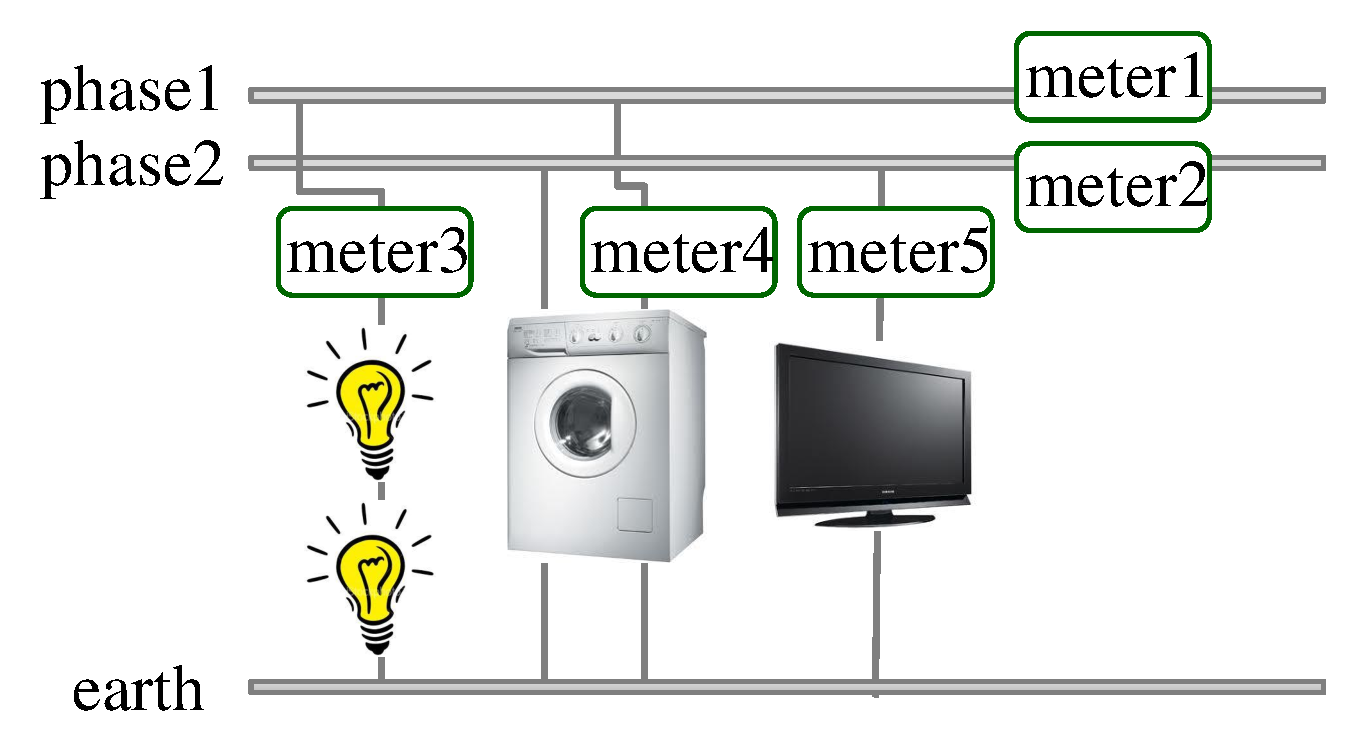
\includegraphics[width=2.5in]{figs/meters.pdf}
%%\caption{Meters on Phases and Circuits}
%%\label{fig_meters}
%%\end{figure}
%For each phase or circuit, meters can be installed
%to record the voltage or current value by voltage
%meter and ammeter.
%Real power is measured by wattmeter.

When meters are installed to monitor the voltage and current,
generally two kinds of data are collected:
low-frequency data and high-frequency data.

In North America, the basic frequency of voltage or current is
60 Hz. 
If the interval between successive data points is larger than 1/60s, 
the data recorded by the meter is low-frequency data; otherwise it is 
high-frequency data. 
High-frequency data can recover the waveform, as
illustrated in Figure~\ref{fig_threephase}.
In practice, only the apparent power
or real power is measured for low-frequency data.
For high-frequency data,
normally current and voltage are monitored separately to facilitate the capture of different device characteristics.
To capture high-order harmonics, the sampling frequency used to record the data
should be at least twice as much as the highest frequency.
When targeting to capture harmonics with the highest order $N_{highest}$, 
 the desired harmonics frequency is $N_{highest} \times 60 Hz$,
then the sampling frequency of recorded data $f$ should
meet the criteria $f \geq N_{highest} \times 1/60 Hz$. 
%\manishc{needs to be fixed} \huijuanc{done.}
%For instance, if the $11th$ harmonics is the highest order 
%we want to use, the recording frequency should be larger than $660$ Hz,
%or $1/660$s.

There are many meters that can record the low-frequency power.
However, high-frequency data must be monitored by special devices such as a TED~\cite{meterTED}.
%\manishc{provide ref.}\huijuanc{done.}
Some examples of aggregated energy data collection include
~\cite{berges2010enhancing}, where a voltage/current meter is installed in a residential
home in Pittsburgh, PA.
This experiment chooses 17 on-off devices and installs plug-level meters for
these 17 devices. 
The data is recorded at a high frequency
(100 kHz). Then features such as real and reactive power and harmonics
are extracted at the frequency of 20 Hz.
Voltage noise data~\cite{patel2007flick} is obtained 
at a high-frequency sampling rate by
plugging the meters into an outlet. Reference~\cite{baranski2003nonintrusive} installs an
optical sensor 
%\manishc{what's an optimal sensor?}\huijuanc{optical other than optimal} 
to collect the real power. Then the on-off events are extracted 
from the real power.
A detailed comparison of
a whole-house meter, circuit meters and plug-meters 
is given in~\cite{berges2010enhancing}.


%\cite{froehlich2011disaggregated} lists what frequency are needed for
%each kind of features as Figure\ref{fig_setup_froehlich2011disaggregated}.
%http://www.theenergydetective.com/how-does-ted-work
%No matter the voltage or current is recorded
%in high frequency or low frequency,
%the instantaneous values are recorded.
%Therefore the steady states,
%which corresponds to power levels
%conform to Gaussian distribution.
%More concisely, if there's average
%value of a power level $\mu$ and
%$\mu=V_{\mu}$, then
%\begin{displaymath}
%(1-\sqrt2\times V_\mu)\leq \mu \leq (1+\sqrt2)\times V_\mu
%\end{displaymath}
%
%To test whether energy disaggregation succeeds or not,
%proper data needs to be obtained.
%Some datasets are obtained by simulation in experiments.
%But majority of devices are gathered by setting
%experiments.
%Table \ref{tb_setup} lists the devices,
%recorded frequency, extracted features for each paper.

%\begin{figure}[ht]
%\centering
%\includegraphics[width=3 in]{figs/noiseflicker.png}
%\caption{Our prototype system consists of a power line noise analyzer plugged in to an ordinary
%wall outlet and connected to a PC (Courtesy:\cite{patel2007flick}).}
%\label{fig_noiseflicker}
%\end{figure}
%
%\subsubsection{EMI}
%\begin{figure}[ht]
%\centering
%\includegraphics[width=3 in]{figs/installationElectriSense.png}
%\caption{Block diagram of major components of ElectriSense (Courtesy:\cite{gupta2010electrisense}).}
%\label{fig_installationElectriSense}
%\end{figure}

\subsubsection{Public datasets}
Although there are many data sets available for energy disaggregation, 
especially in the power industry, 
the majority of them are not open to the public. 
So far there are a few public data sets, including REDD~\cite{kolter2010redd},
BLUED~\cite{anderson2012blued}, Smart~\cite{barker2012smart}, 
AMPds~\cite{makonin2013ampds}, CASAS~\cite{cook2013CASAS}, iAWE~\cite{batra2013different}, 
and GREEND~\cite{monacchi2014greend}. %(? compare more according to GREEND papers)
The first open data set REDD, when introduced, opened the doors for several 
researchers to attack the energy disaggregation problem.

So far, a majority of this data is stored as plain text. 
Some work proposes to store these datasets in a database~\cite{lai2012database}  
or builds a metadata as a standard~\cite{kelly2014metadata}. 


%\subsection{Features Summary}
%To disaggregate devices from aggregated current, voltage, or power data,
%we need to first understand the basic features of electrical devices.
We introduced
some of these features in Section~\ref{sec:basic} such as voltage, current, real power, 
reactive power, harmonics generated by current and voltage. Some more basic and 
derived features
include: startup of current; waveform of current;
wavelet of current waveform; eigenvalue of current waveform;
voltage waveform; voltage noise; EMI
by gauging noise; electromagnetic field around the devices; 
duration time of power levels by calculating current and voltage; 
and time correlation of devices. 

%The features that can be extracted from a data set 
%depend on the installed meters 
%and the sampling frequency of data recording. 
%Current meter and voltage meter can show current and voltage values
%at the sampling points.
%If the sampling frequency is high enough, larger than several hundreds Hz,
%the waveform of current or voltage can be reconstructed.
%The noise data is recorded by a special plug-in meter, which is installed in some power 
%outlets instead of being installed on main service current or voltage electrical lines.

%combination of two
%\begin{figure}[h]
%\centering
%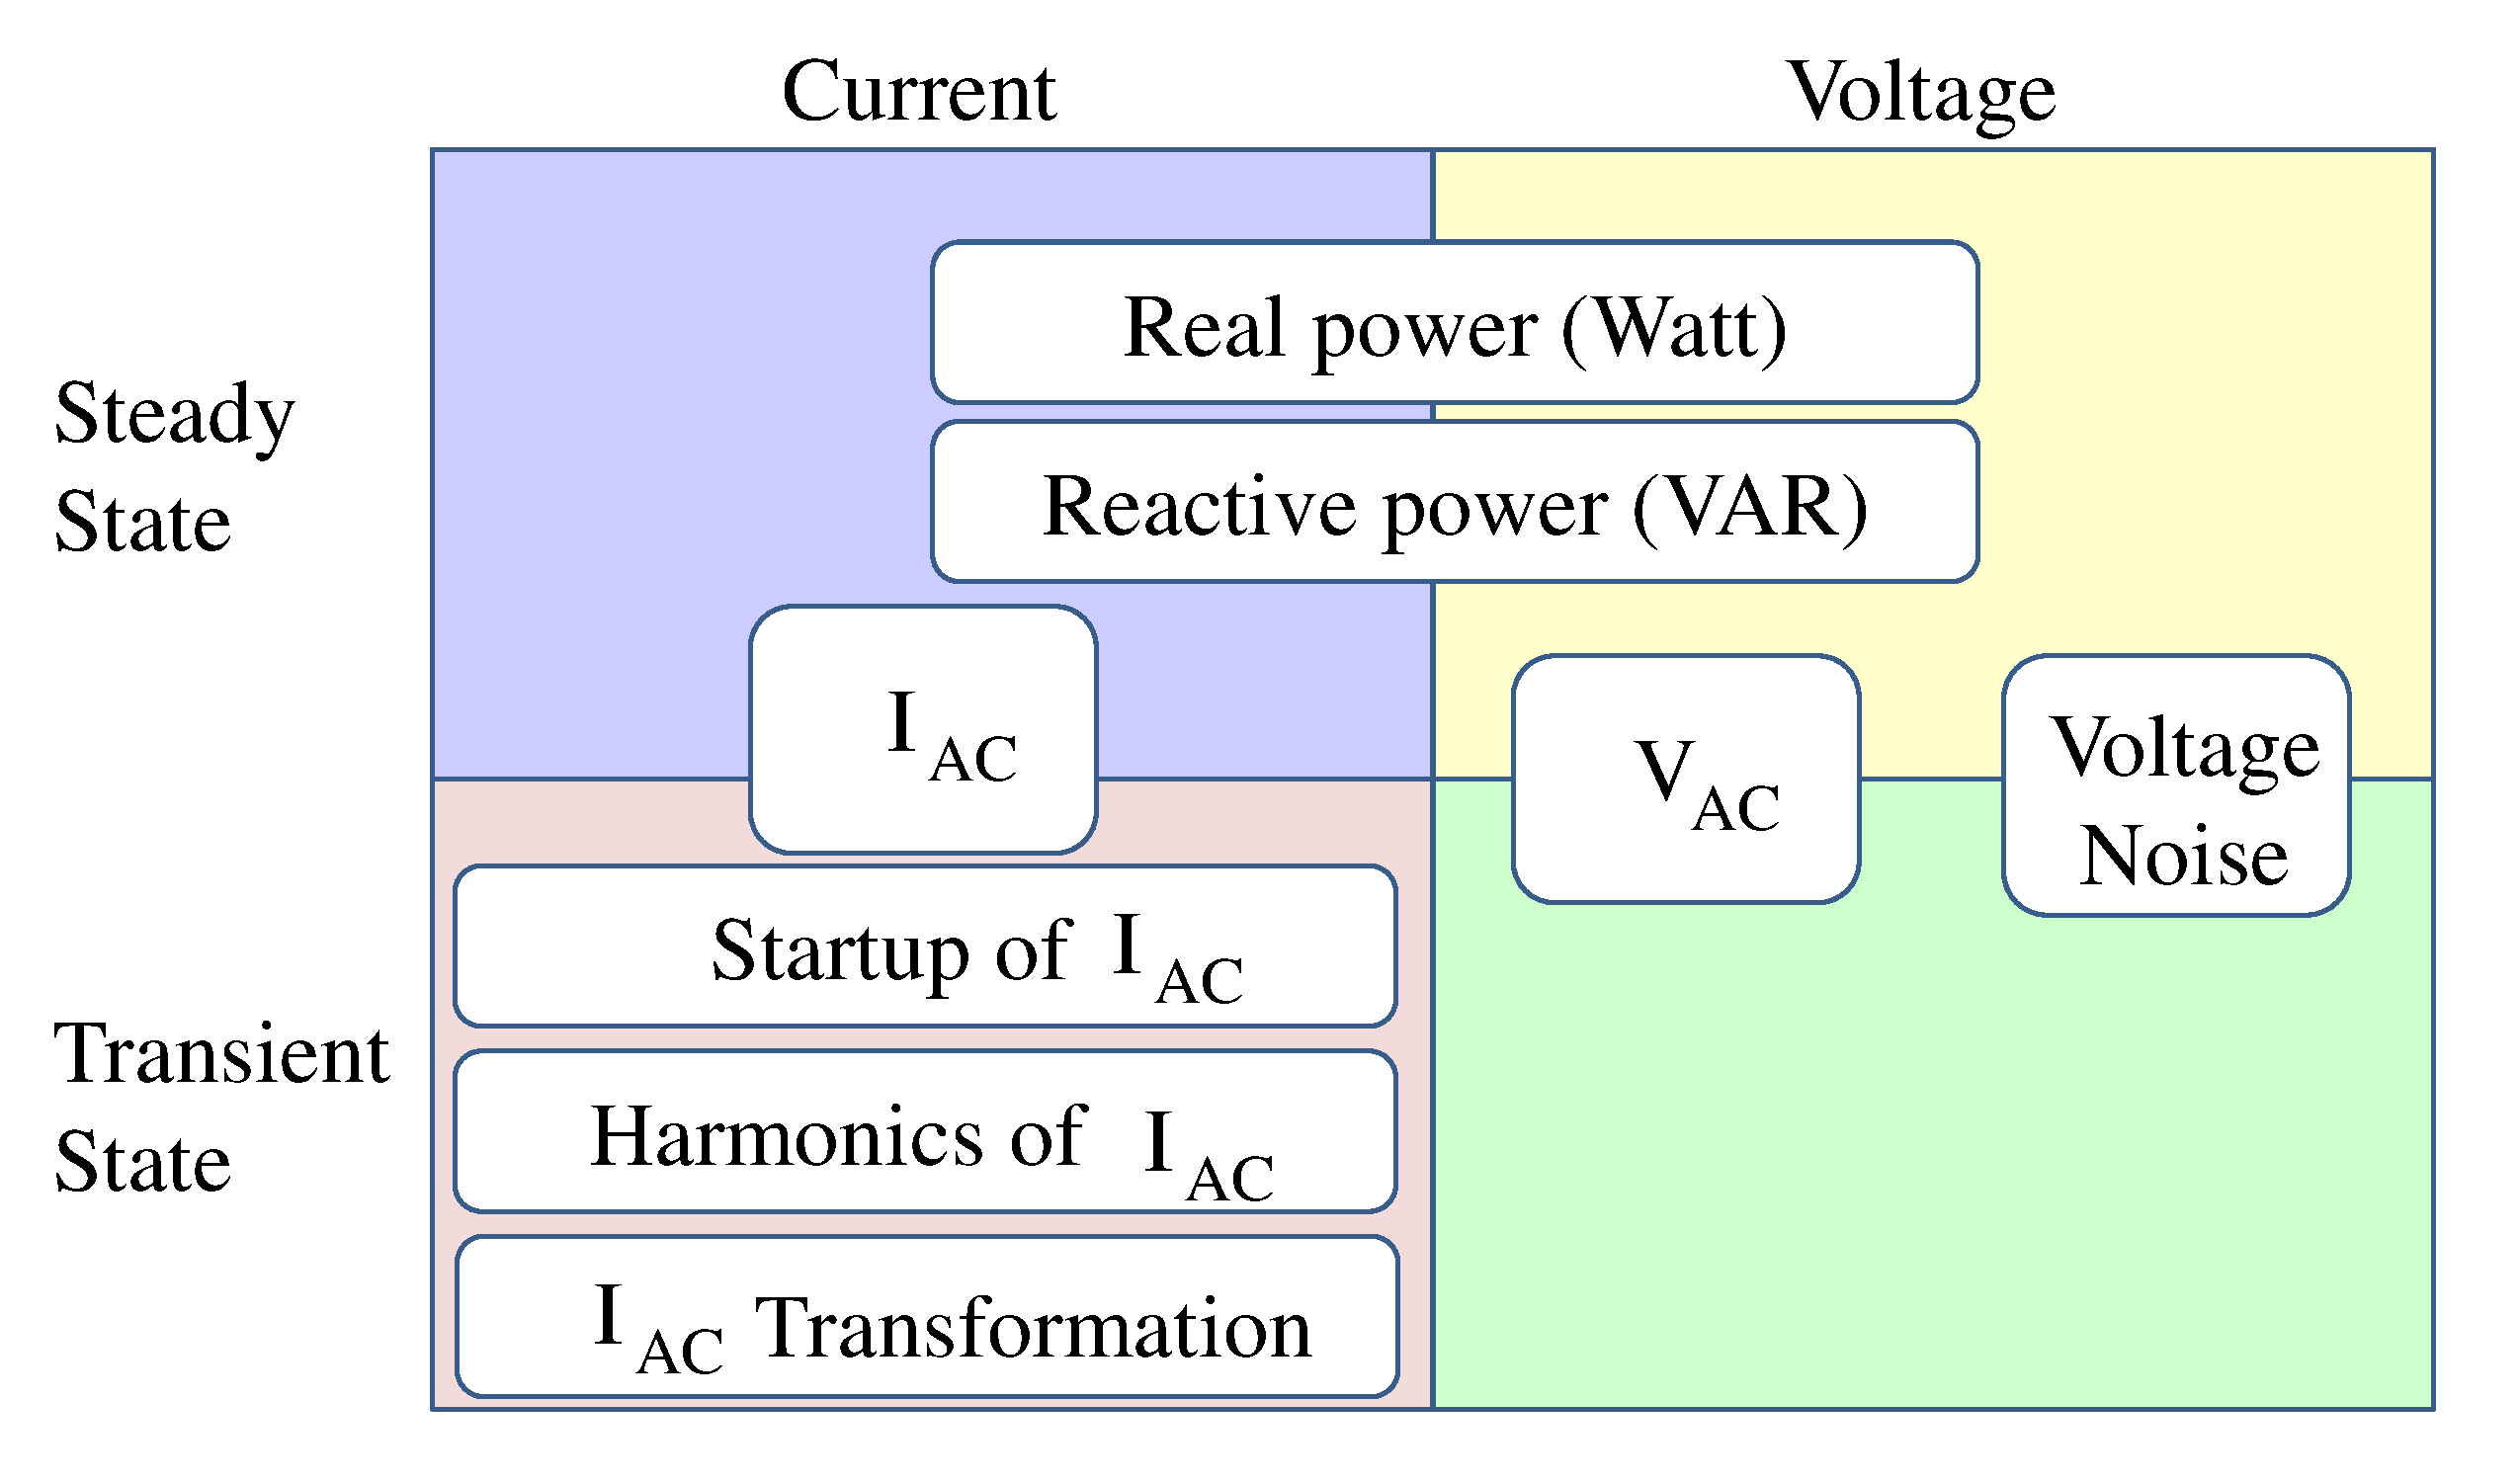
\includegraphics[width=3 in]{figs/fig_acpower.pdf}
%\caption{Category of AC Power Features}
%\label{fig_ACPowerFeatures}
%\end{figure}

%\begin{figure}[h]
%\centering
%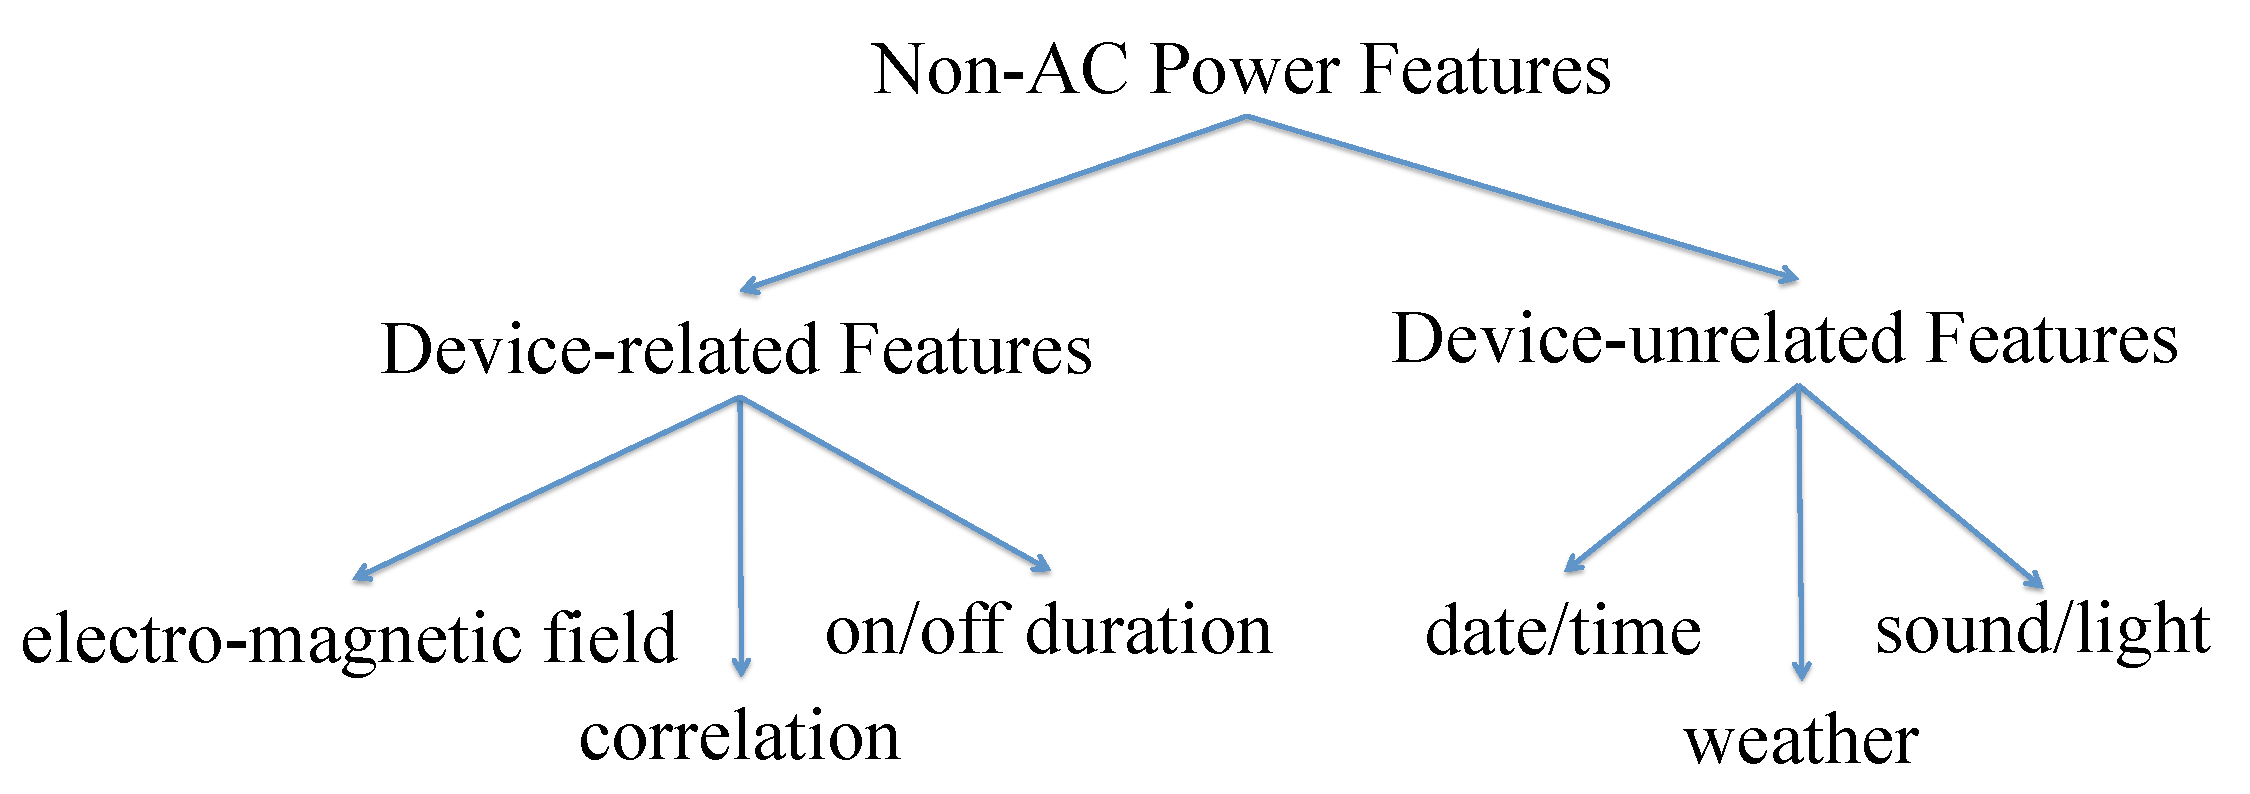
\includegraphics[width=3.5in]{figs/NonPowerFeatures.pdf}
%\caption{Category of AC Power Features}
%\label{fig_NonACPowerFeatures}
%\end{figure}

\begin{figure*}[h]
	\centering{
    \begin{tabular}{cc}
    	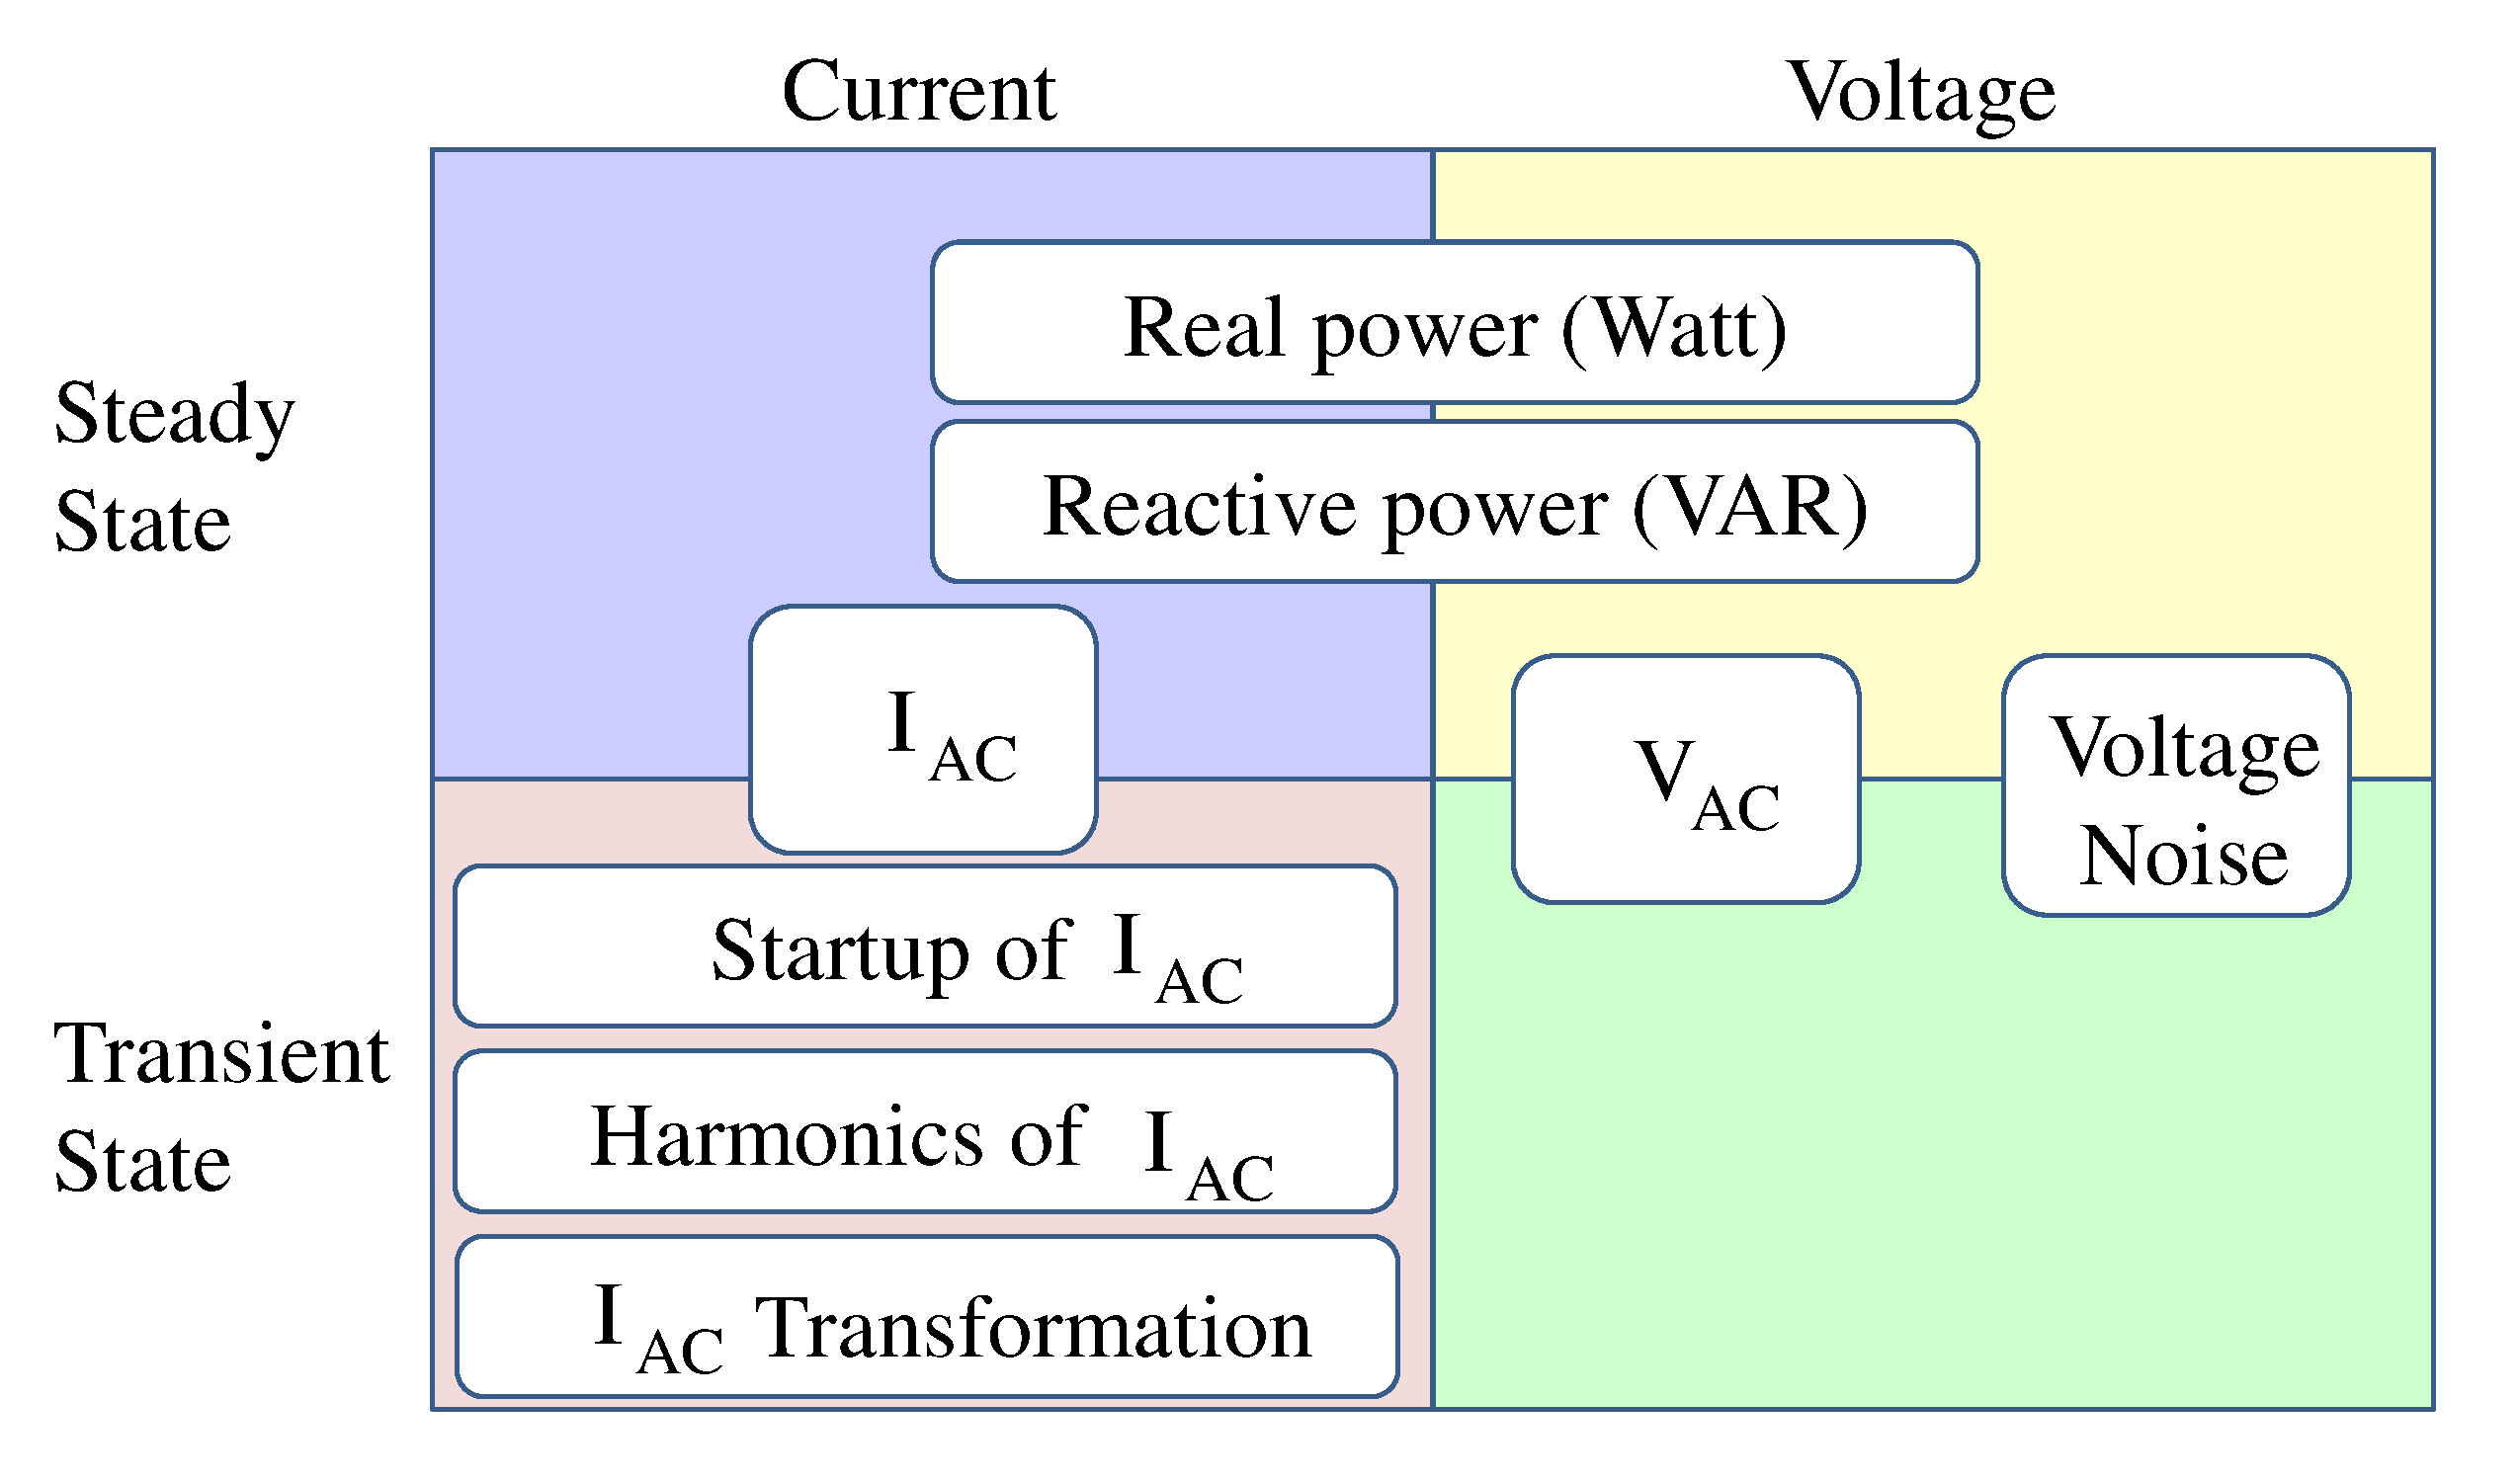
\includegraphics[width=0.45\textwidth]{figs/fig_acpower.pdf} \hspace{1em}&	
	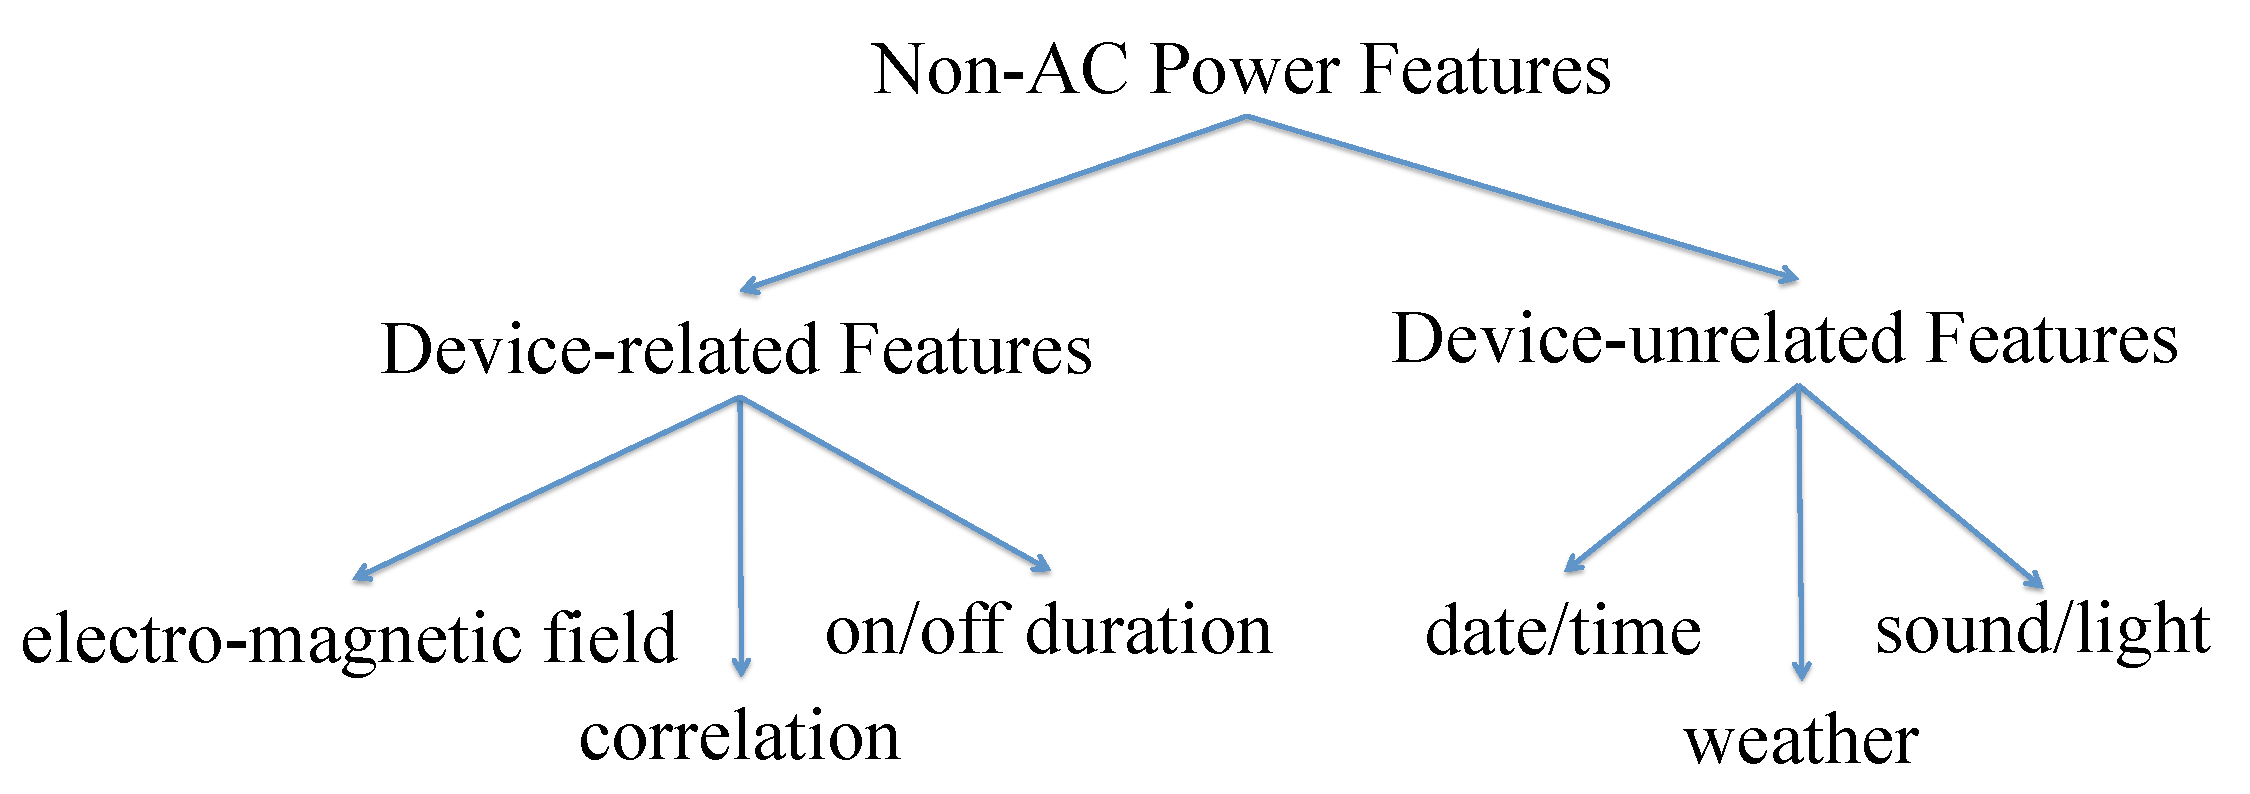
\includegraphics[width=0.55\textwidth]{figs/NonPowerFeatures.pdf} \tabularnewline
    \end{tabular}
    }
	\caption{Category of (a) AC Power Features and (b) Non-AC Power Features. }
	\label{fig_ACPowerFeatures}
\end{figure*}
	

Figure~\ref{fig_ACPowerFeatures} (a) displays a classification of AC power features.
AC power features are related to current or voltage.
These features can also be classified based on the stability of operating states.
(In the below, a
steady state refers to the stable state after a device turns on.)
For example, real power, reactive power, and apparent power
are all steady state features.
Transient states refer to variable states during a very
short period of time when a device turns on or off.
Transient state features are generally derived from
the startup shape of current, voltage,
harmonics or harmonics transformations.
%\begin{figure}[h]
\centering
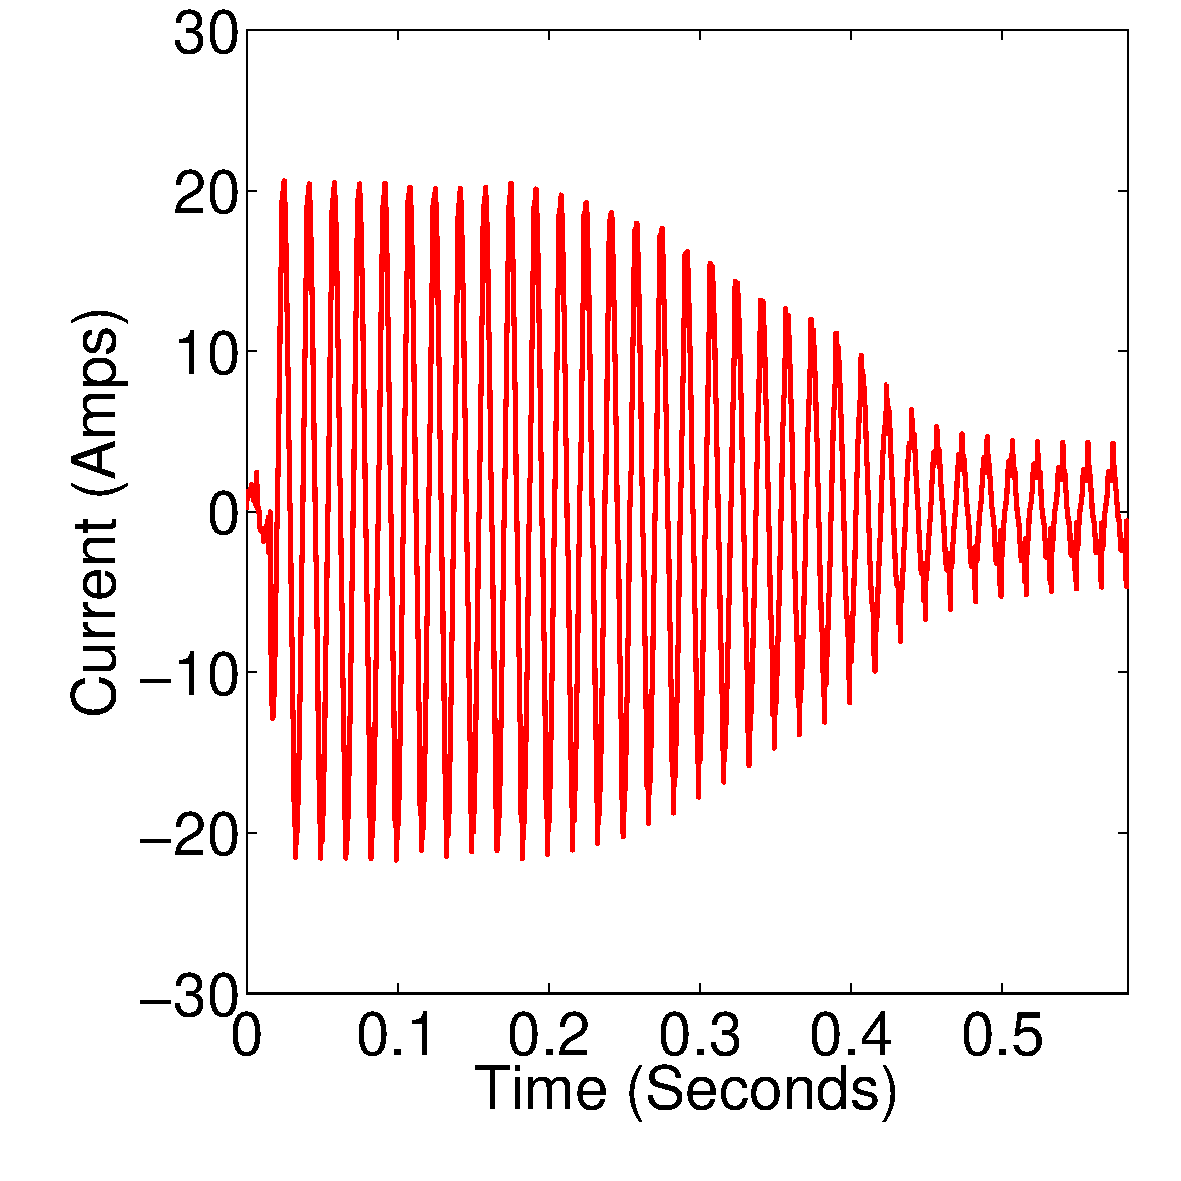
\includegraphics[width=2.5 in]{figs/refrigeratorTransient.pdf}
\caption{Transient and Steady State of a Sinusoidal Current from a Refrigerator.}
\label{fig_transientexample}
\end{figure}

%Any current or voltage is the sum of a transient state 
%and steady state as a function of time. 

Non-AC power features are summarized in %Table. \ref{tab_nonacpower}.
Figure~\ref{fig_ACPowerFeatures} (b). 
%Figure\ref{fig_NonACPowerFeatures}. 
%\begin{figure}[h]
\centering
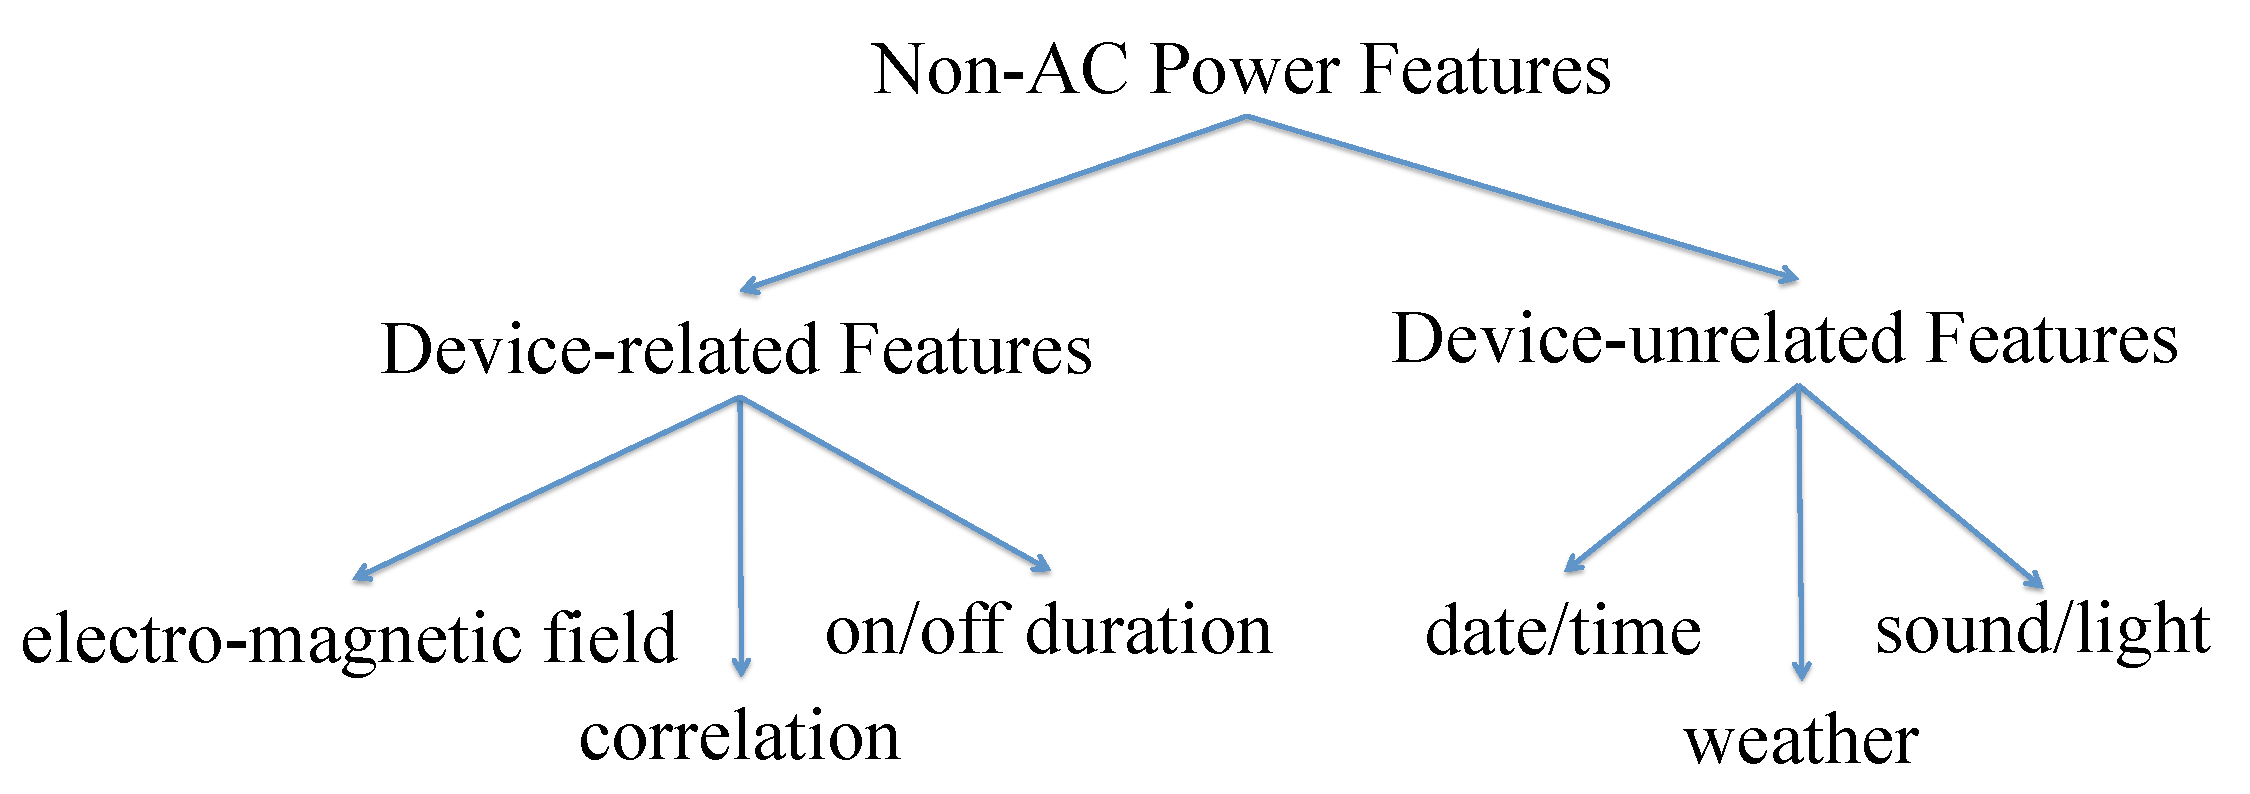
\includegraphics[width=3.5in]{figs/NonPowerFeatures.pdf}
\caption{Category of AC Power Features.}
\label{fig_NonACPowerFeatures}
\end{figure}

These non-AC power features can be classified into two categories:
device-related and device-unrelated. 
%\manishc{call these device-related and device-unrelated features}\huijuanc{ok.Done.}
Device-related category includes electromagnetic field (EMF); 
operational information such as on/off durations, and
 correlation between devices.
%\manishc{where is on/off duration of a device used as a feature?}  
%\huijuanc{in the paper of \cite{kim2011unsupervised}, the on/off duration is used in the semi-FHMM Model.}
The EMF is produced when certain devices are on. 
The device-unrelated category is comprised of 
date or time features, such as month of the year,
day of the month, day of the week and time of the day.  
Also, it includes the ambient temperature, which
plays a crucial role in determining the functioning
of the HVAC system.
%When the weather is hot outside - the cooler is turned on and in
%the cold season the heater is used. 
Further the device-unrelated category include features like sound and 
light produced by an electrical device. 
A sensor can be installed near a device 
to record such features.  

\subsection{AC Power Features}
\subsection{Steady state}
\iffalse
\huijuanc{comment out until huijuan's next comment}
As shown in Figure~\ref{fig_ACPowerFeatures}, 
steady state features include real and reactive power from both 
low frequency and high frequency data, 
current or voltage from high frequency data, 
and voltage noise. \manishc{figure 11 doesn't show anything about high/low frequency} 
\huijuanc{agree. rewritten as follows.}
\fi
As shown in Figure~\ref{fig_ACPowerFeatures}, 
steady states include real power, reactive power, 
current, voltage, 
and voltage noise. 
This data can be either read directly from meters
sampled at low frequency or calculated indirectly from 
high frequency voltage and current data. 
\iffalse
\manishc{in this sentence, are
  you saying the meters that sample at low frequency compute the real/reactive
  power, while the meters that sample at high frequency do not?} 
  \huijuanc{Yes, this is what I mean. Is it correct?}
\fi  
Suppose the basic current/voltage frequency of
AC power, $\omega$, is 60 Hz
and the sampling frequency of recorded data is $f$,
i.e., there are in total $f/60$ number of sample points in
each cycle.
The real power value is the average product
of current and voltage in a cycle as in Equation (\ref{eq_realpowerhighfreq}). 
\begin{equation}
P_{av}= \frac{\sum_{t}^{t+f/60} v(t) \cdot i(t)}{f/60}
\label{eq_realpowerhighfreq}
\end{equation}
%When introducing the angle phase difference between current and voltage, 
%we can also calculate the instantaneous reactive power according to 
%Equation (\ref{eq_powerTriangle}) in section~\ref{sec_pvCalculation}.
%\manishc{how do you compute the reactive power from that equation? It has
 % apparent power as well, where do you get that from?}

Real power is the most basic feature and used 
by almost all prior work in energy disaggregation \cite{hart1992,powers1991using,farinaccio1999using,marceau2000nonintrusive,baranski2004genetic,baranski2004detecting}.
Reactive power is also widely used as a feature, e.g., in \cite{hart1992,laughman2003power,drenker1999nonintrusive}.
Figure~\ref{fig_realReactive_hart1992} shows real power and 
reactive power features of different devices. 
For some devices real and reactive power are sufficient to distinguish
between them. 
A refrigerator and water pump have similar reactive power but
different real power; thus using the real power feature, we can separate them. 
A refrigerator and garage door opener have similar real power but different reactive power;
thus the reactive power is the distinguishing feature in this case.
Steady state features are also derived from the variations of real or reactive power.
For instance, in~\cite{milioudis2013event}, 
the slopes of both active and reactive power 
are extracted as vectors. % as shown in Figure\ref{fig_ACPowerFeatures}. 


\subsection{Transient state}
High frequency data, 
from which the current waveform or voltage waveform can be recovered, 
%\manishc{what does
%  ``reconstructed'' mean here; you are already measuring current/voltage at
%  high frequency. You may want to reword/explain.}\huijuanc{I mean the waveform of the current 
%  or voltage can be reconstructed. }
offers rich features that can be applied to energy disaggregation. 
These features include the startup of current, 
harmonics of current, 
harmonics of voltage, 
voltage noise and its transformations. 

\textit{Startup duration and transient power:}
Startup duration and transient power are recorded when a device is turned on. 
Usually a non-linear device, like a microwave, has such a distinguishing feature.
%\manishc{not clear what this means, please re-word}.    
When this kind of device turns on,
the power usage usually changes to a temporary high value for few 
or milliseconds, %\manishc{this is too high! do you mean millisec?}\huijuanc{yes. already updated}, 
then jumps into a steady state for a longer time.
This temporary startup duration and shape feature varies from one device to another. 
Comparing the transient power changes with the steady state, 
the trail of power changes against time looks like a spike or a curve with changing slope. 
Figure~\ref{fig_realTransient} shows examples of current, average real power and instantaneous
real power in the first 0.5 seconds of a refrigerator turning on in the 
BLUED dataset~\cite{anderson2012blued}. 
\iffalse
 \manishc{you said 0.5 sec in the previous
  sec; make it consistent, and this sentence seems like a repetition} \huijuanc{updated, and remove the repeated sentence}. 
\fi  
In Figure~\ref{fig_realTransient} (a), there are three areas in this waveform.
When $0<t<0.02s$, the current is in
a steady state.
When $0.02s \leq t \leq 0.45s$,
the current is in a transient state,
during which the amplitude of the current changes
rapidly. 
%\manishc{the amplitude of the current is changing, but the frequency
 % doesn;t seem to change much.}\huijuanc{agree. updated.}
When $ t \geq 0.45s$, the current comes again to a
steady state.
Figure~\ref{fig_realTransient} (b) shows the shape of corresponding average power. 
\iffalse
\manishc{i assume this is average power? please call it average power,
  since you are talking about instantaneous power here as well} \huijuanc{done.}
It reaches around 400 watts for a very short period of time 
\manishc{i don;t
  see it being 400 W in fig 12 (b)}\huijuanc{deleted}
\fi 
It jumps to 1600 watts in a very short period of time, then gradually decreases to 200 watts (calculated using
Equation (\ref{eq_realpowerhighfreq})).
Figure~\ref{fig_realTransient} (c) depicts the instantaneous real power. 
There are 200 points in each cycle. As can be seen, the
instantaneous power changes very frequently.
\begin{figure*}[ht]
	\centering{
    \begin{tabular}{ccc}	
    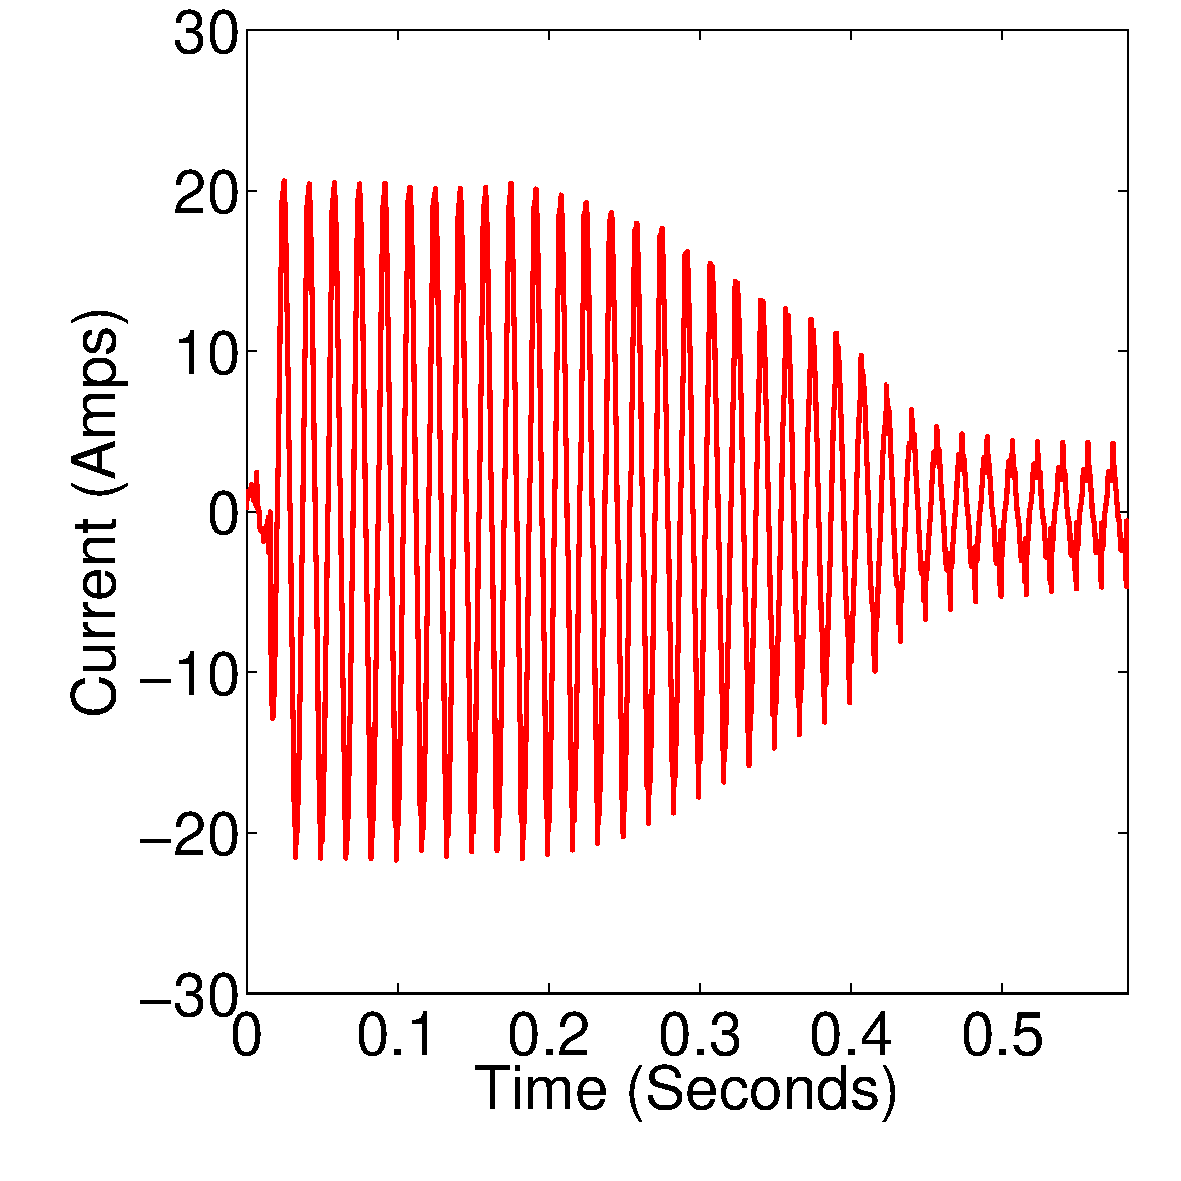
\includegraphics[width=0.29\textwidth]{figs/refrigeratorTransient.pdf}                 \hspace{1em}&
    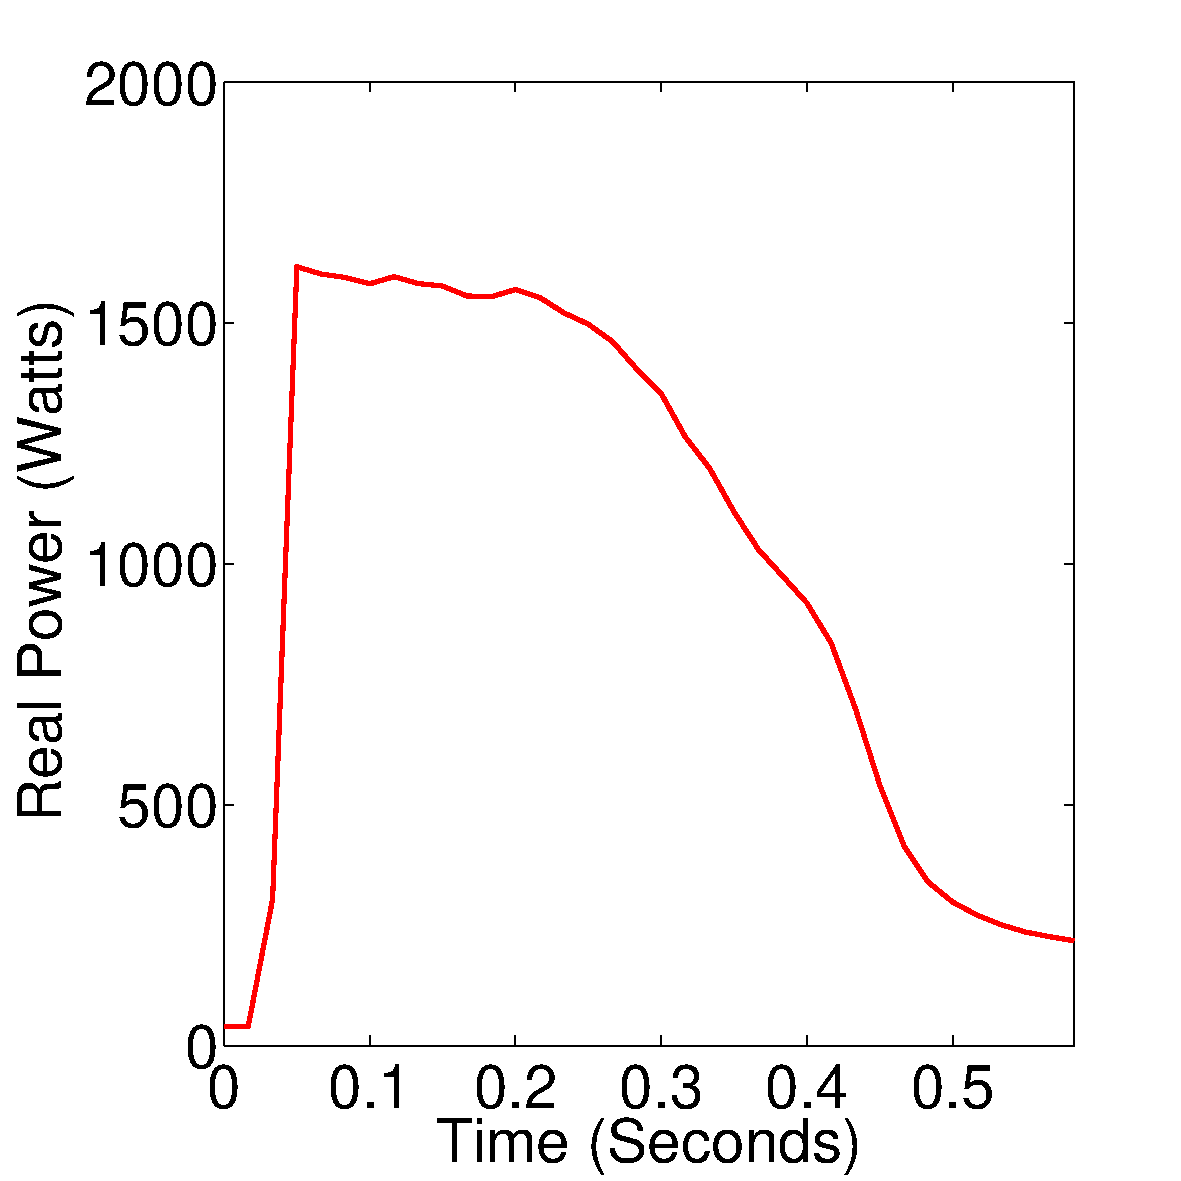
\includegraphics[width=0.3\textwidth]{figs/refrigeratorTransientRealPower.pdf} \hspace{1em}&
    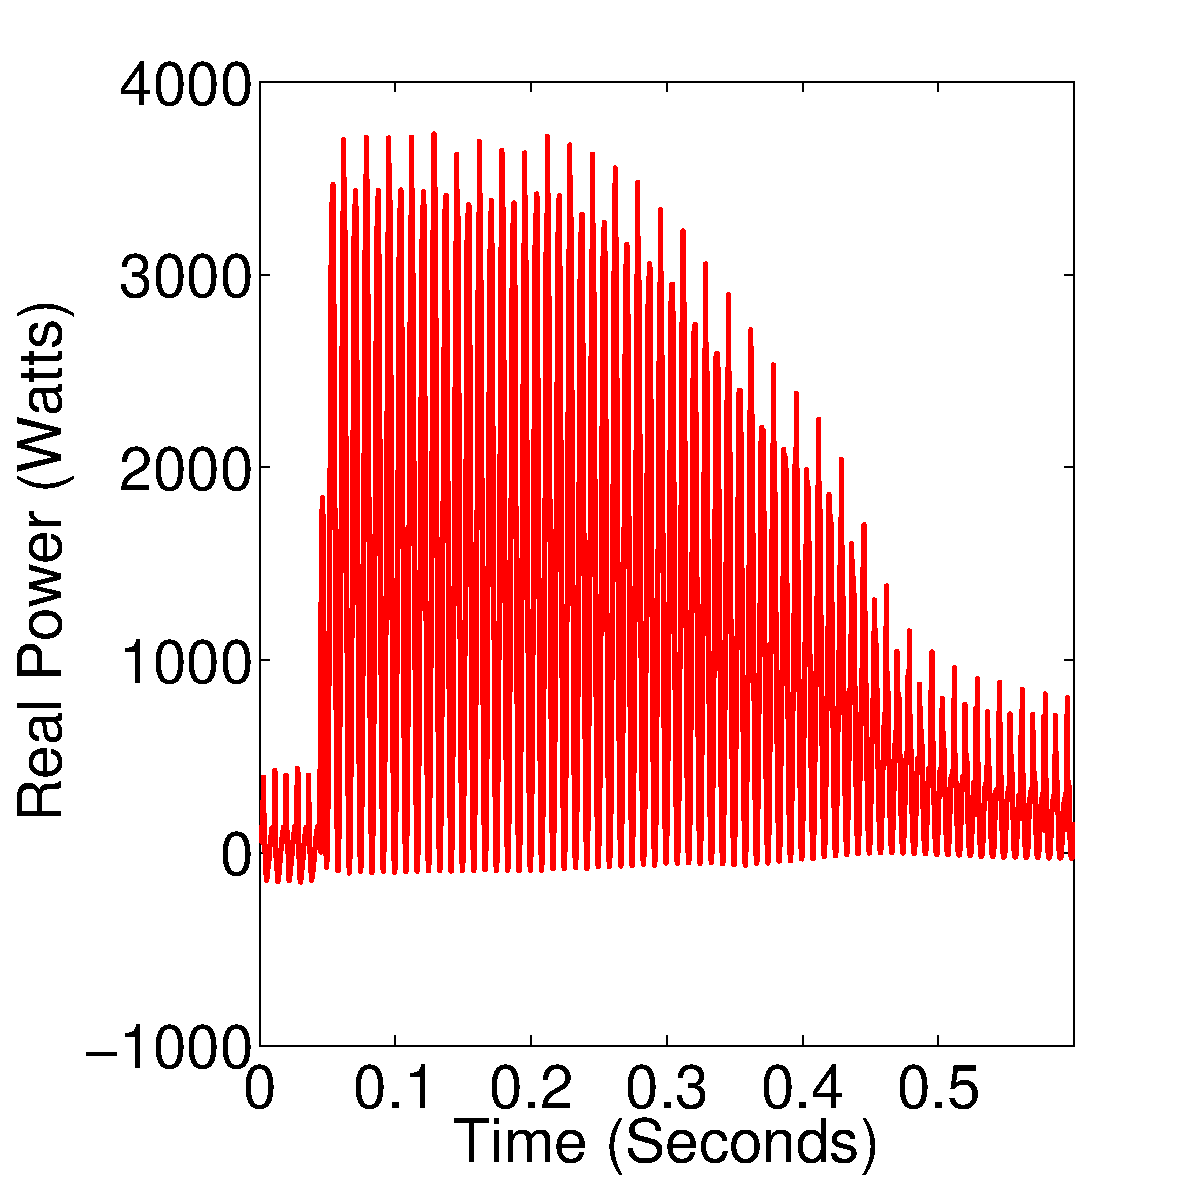
\includegraphics[width=0.3\textwidth]{figs/refrigeratorTransientInstantPower.pdf} \tabularnewline
    (a) & (b) & (c)\tabularnewline
    \end{tabular}
    }
	\caption{(a) Transient and Steady State of a Sinusoidal Current from a Refrigerator. Transient Shapes for a Refrigerator (b) Real Power and (c) Instantaneous Real Power.}
	\label{fig_realTransient}
\end{figure*}

%transient.tex
%\begin{figure}[h]
%\centering
%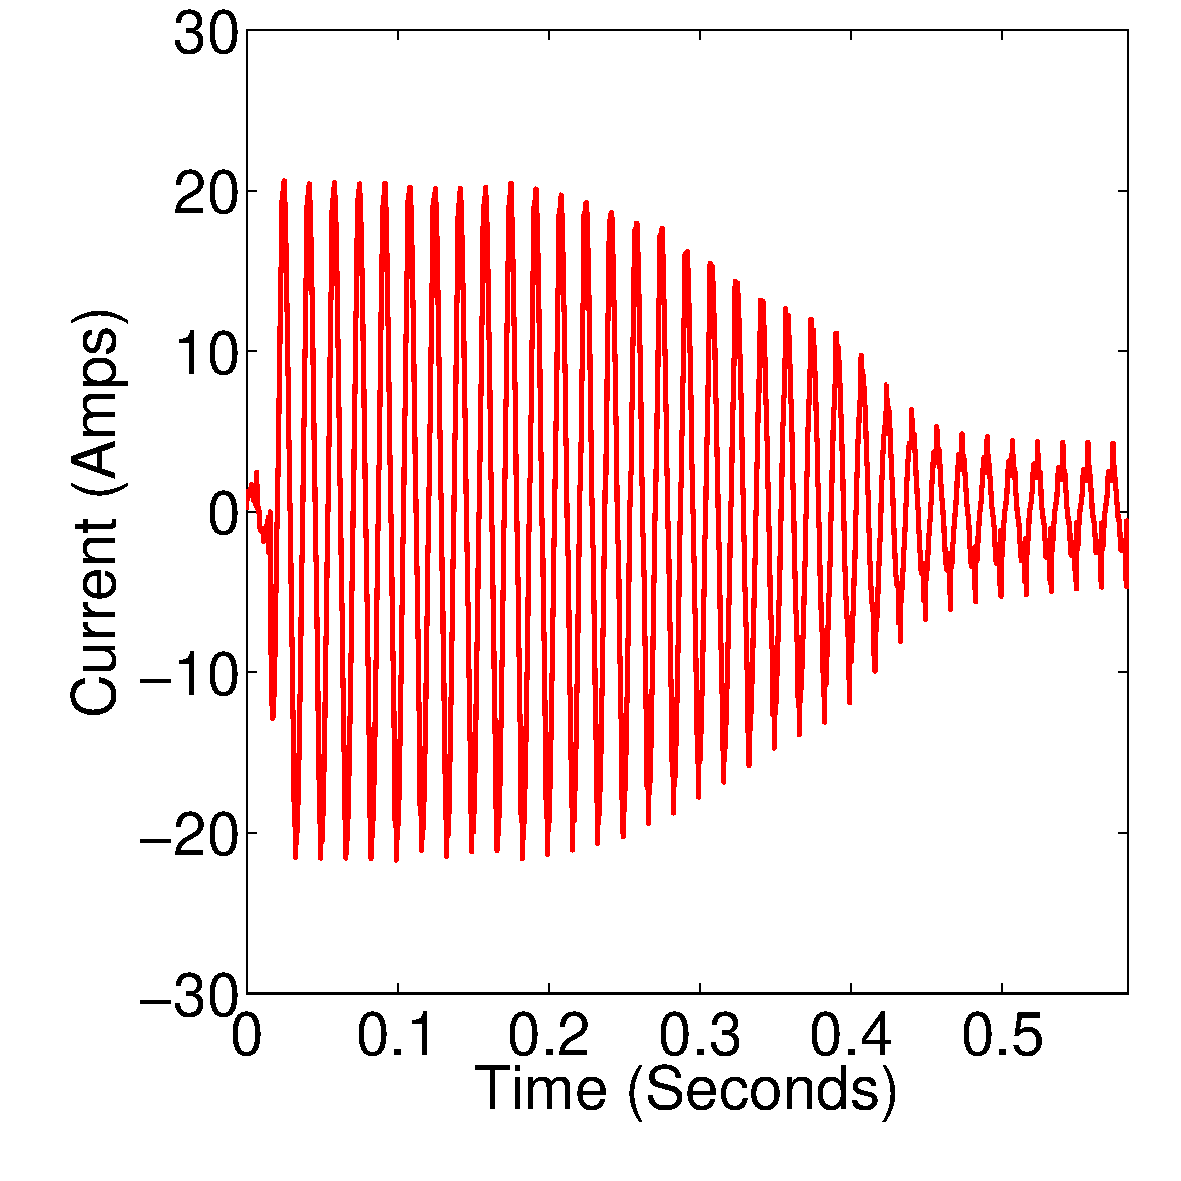
\includegraphics[width=2.5 in]{figs/refrigeratorTransient.pdf}
%\caption{Transient and Steady State of a Sinusoidal Current from a Refrigerator.}
%\label{fig_transientexample}
%\end{figure}

The transient energy %\manishc{real power?} \huijuanc{change power as energy} 
is calculated as 
$E_{transient} = \int_{t_s}^{t_s+\delta t} v(t)i(t)dt $, 
where $t_s$ is the start time and $\delta t$ is the startup duration. 
The corresponding real power is calculated as 
$P(t) = \frac{dE_{transient(t)}}{dt} = v(t)\cdot i(t)$.
\iffalse
\manishc{this is confusing, is ``transient power'' ``transient real power''?
  what is the unit of transient power? is it Watts? from your equation of
  $P_{transient}$ it appears to be Watt Second? can you verify these
  equations, and explain how transient power is different from real power. I
  initially thought that transient power is just the power during the
  transient period; is that correct?}\huijuanc{already verified the equation and changed it.}
\fi  
%\begin{eqnarray*}
%W_{transient} = \int_{t_s}^{t_s+\Delta t} v\cdot i \cdot dt \\
%\end{eqnarray*}

This startup duration and shape of current or power feature can be used 
standalone or in integration with other features.
~\cite{sultanem1991using} gives a typical example of the latter case. 
The startup duration and the shape of current or power feature 
is combined with real power and reactive power
to distinguish each device among refrigerator, washing machine, and fluorescent light.
Note that 
this transient startup may be called transient spectral envelope~\cite{shaw2000PhdThesis}, 
or transient power. 
%It has been applied in previous work
%as features to identify electrical device.(?give an example)

\textit{Current or voltage waveform:}
The current waveform $I_{ac}$, which can be simply read from
high frequency recorded data,
is a typical feature used to discriminate devices.
The waveforms generated by non-linear devices  are 
very different due to the waveform distortion 
introduced by each device. 
Figure~\ref{fig_waveformTraj} (a-b)
illustrates the current waveform 
of two devices---refrigerator and compressor---from the
BLUED dataset. 
From them, we can see that both the magnitudes  and the distortions 
of the current waveforms differ from each other. 
The maximum current magnitude of a refrigerator is 20 Amps while that of 
the compressor is around 16 Amps. 
%\begin{figure*}[ht]
	\centering{
    \begin{tabular}{cc}	
	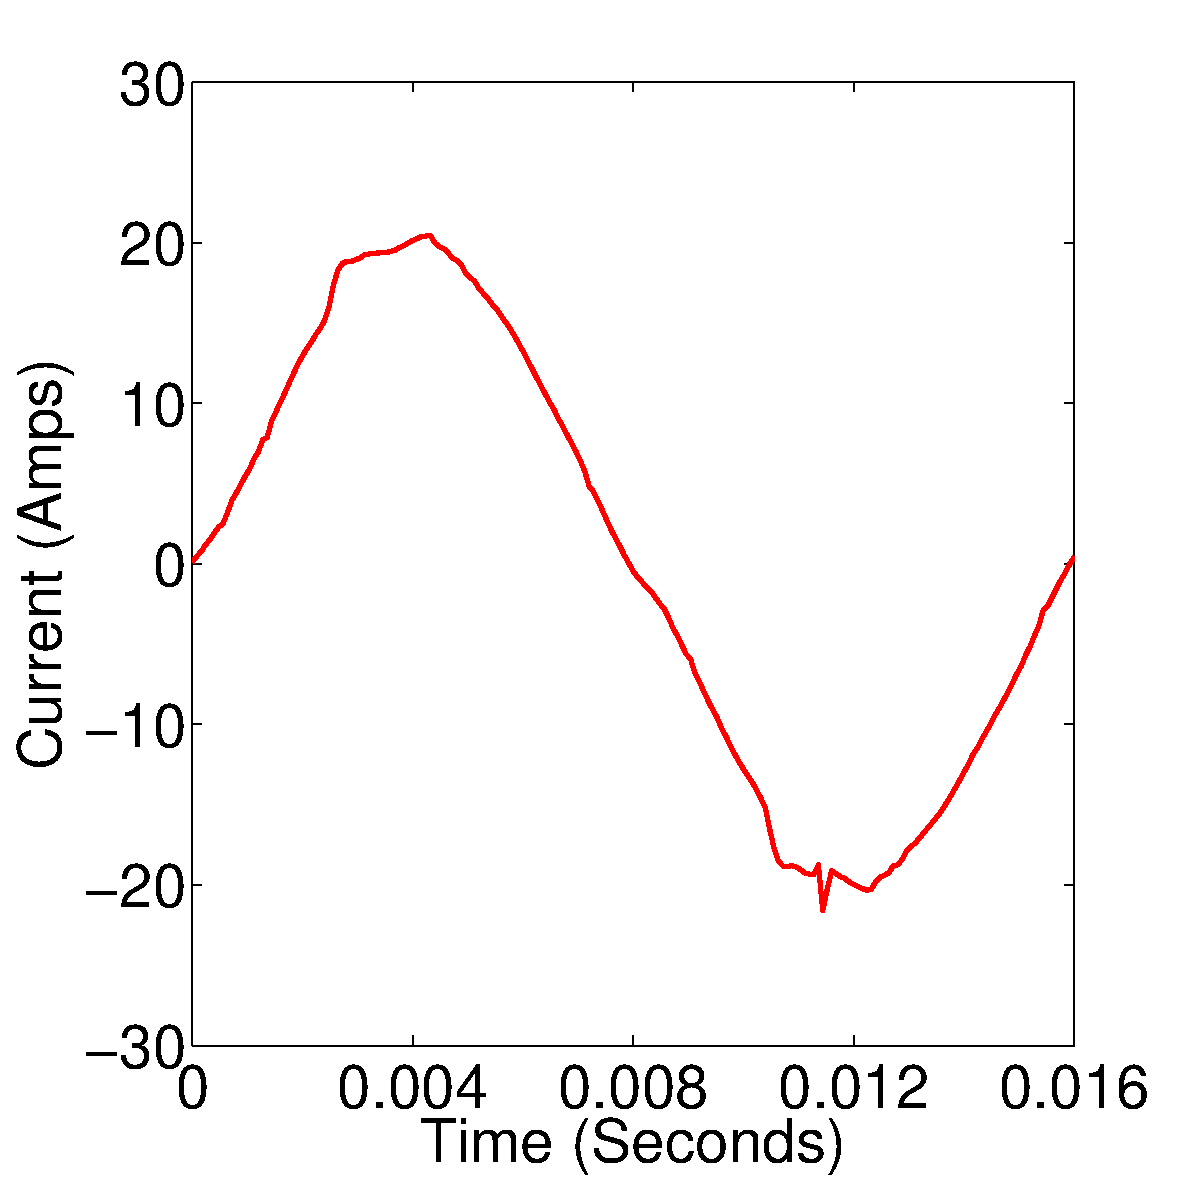
\includegraphics[width=0.5\textwidth]{figs/refrigeratorTransientSingle.pdf} \hspace{1em}&
    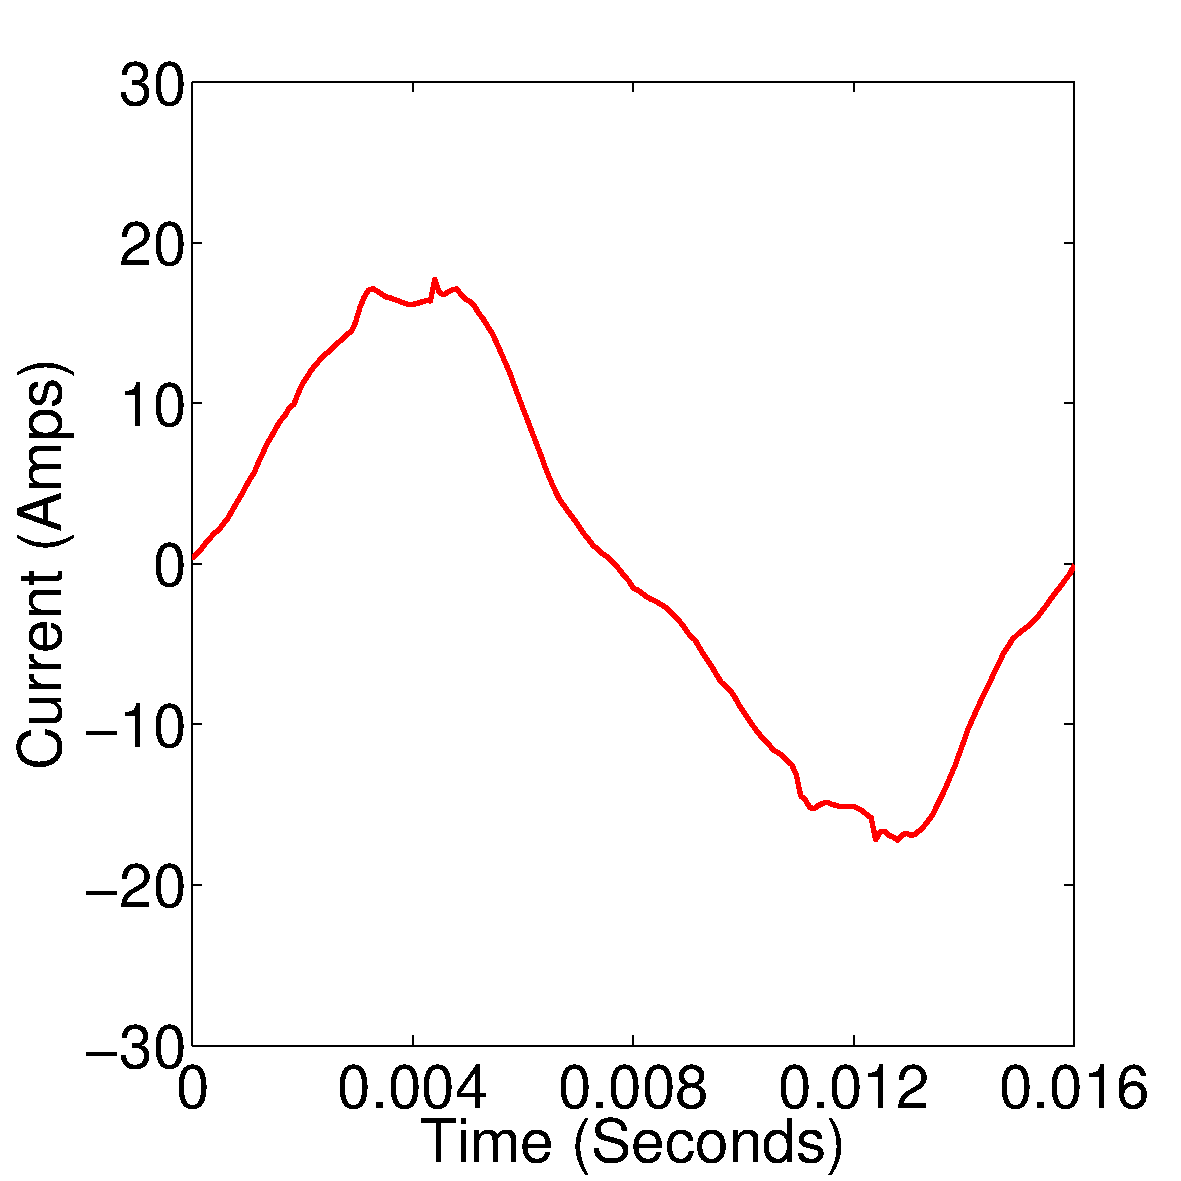
\includegraphics[width=0.5\textwidth]{figs/airCompressorTransientSingle.pdf} \tabularnewline
    (a) & (b) \tabularnewline
    \end{tabular}
    }
	\caption{Current waveform of (a) a refrigerator and (b) an air compressor.}
	\label{fig_currentwaveform}
\end{figure*}
 

Current or voltage waveform features have been applied in previous work.
The unprocessed current waveform 
%just like waveform in Figure~\ref{fig_currentwaveform}, 
is regarded as a feature in~\cite{suzuki2008nonintrusive}.
This paper shows that 
the raw current waveforms of a microwave oven and a toaster oven 
are different in a cycle. 
Therefore, these raw current waveforms can be used to separate 
these two devices. 
However, raw current waveforms are prone to changes with noise.
\cite{duan2004neural} analyze the current waveforms of eight devices and classify
them as A/C, refrigerator, compressor, 
fan (VSD), elevator (converter), elevator (M/G set), fluorescent lights 
and computers. 
Similarly, standalone voltage waveform has been used as a feature in previous work. 
%The distortion is mainly generated by non-linear devices.
By analyzing voltage shapes,
we can determine which device is on.
%The difference of voltage waveform is that the maximum value of 
%voltage is approximately 116V in the U.S.
%\cite{cox2006transient} uses the distortion of voltage waveform to
%separate transient shapes as described in~\cite{srinivasan2006neural}.
While a combination of current and voltage waveforms has been proposed as
features, \cite{hassan2014empirical} show that the disaggregation results 
are better
when adopting either the current waveform or the voltage waveform-based
features exclusively.

In order to overcome the shortcomings of raw current or voltage waveforms, 
several variations or transformations of these waveforms have been proposed. 
The first is the voltage-current (V\-I) or current-voltage (I\-V) trajectory. 
This idea is useful because for
dynamic devices such as an air conditioner,
the current waveform may vary from cycle to cycle.
Figure~\ref{fig_waveformTraj} (e-f) illustrates the current trajectory difference between 
two devices, %\manishc{what is a sequential device?}\huijuanc{not sure. delete sequential}, 
viz a refrigerator and an air compressor in the BLUED dataset. 
From Figure~\ref{fig_waveformTraj} (c) and (d), 
we can see that there is only a slight difference between the current and voltage waveforms.
\iffalse
\manishc{not
  clear, do you mean in subfigures (c) and (d), there is a difference in the
  current and voltage waveforms?} \huijuanc{Yes. I mean little difference not much.}
\fi  
But when comparing the current against the voltage as shown in
Figure~\ref{fig_waveformTraj} (e) and (f), 
the V-I trajectories are quite different. 
 %Circuit4 and dining room light. 
%From it, we can see thtat after the dinning room light is turned on, 
%the current changes some in the first half cycle. 
\begin{figure*}[h]
	\centering{
    \begin{tabular}{ccc}
    	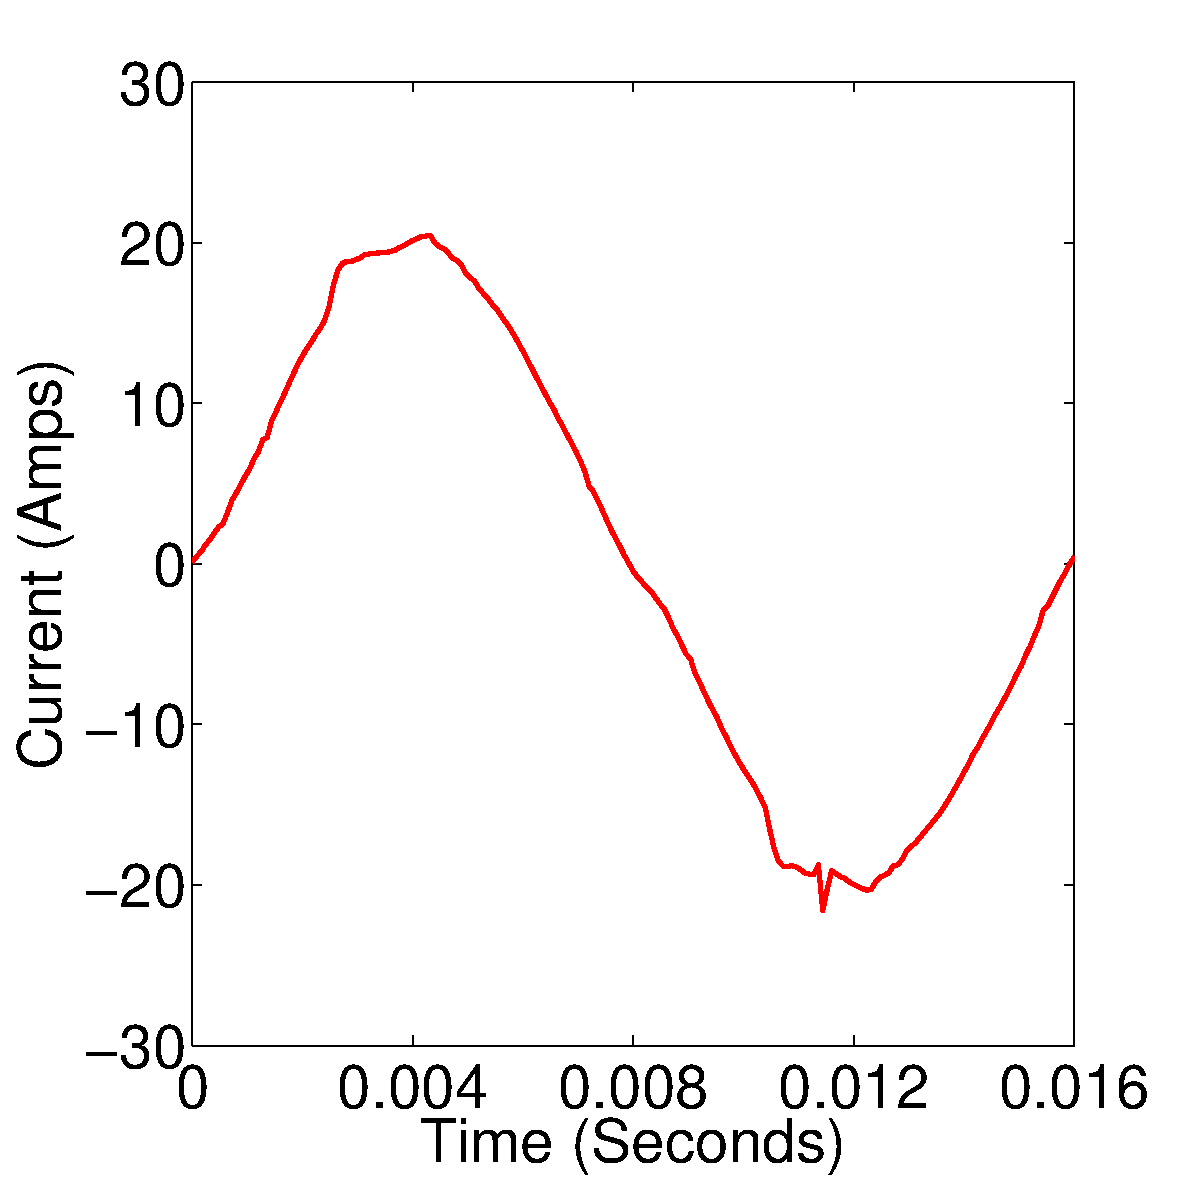
\includegraphics[width=0.3\textwidth]{figs/refrigeratorTransientSingle.pdf} \hspace{1em}&	
	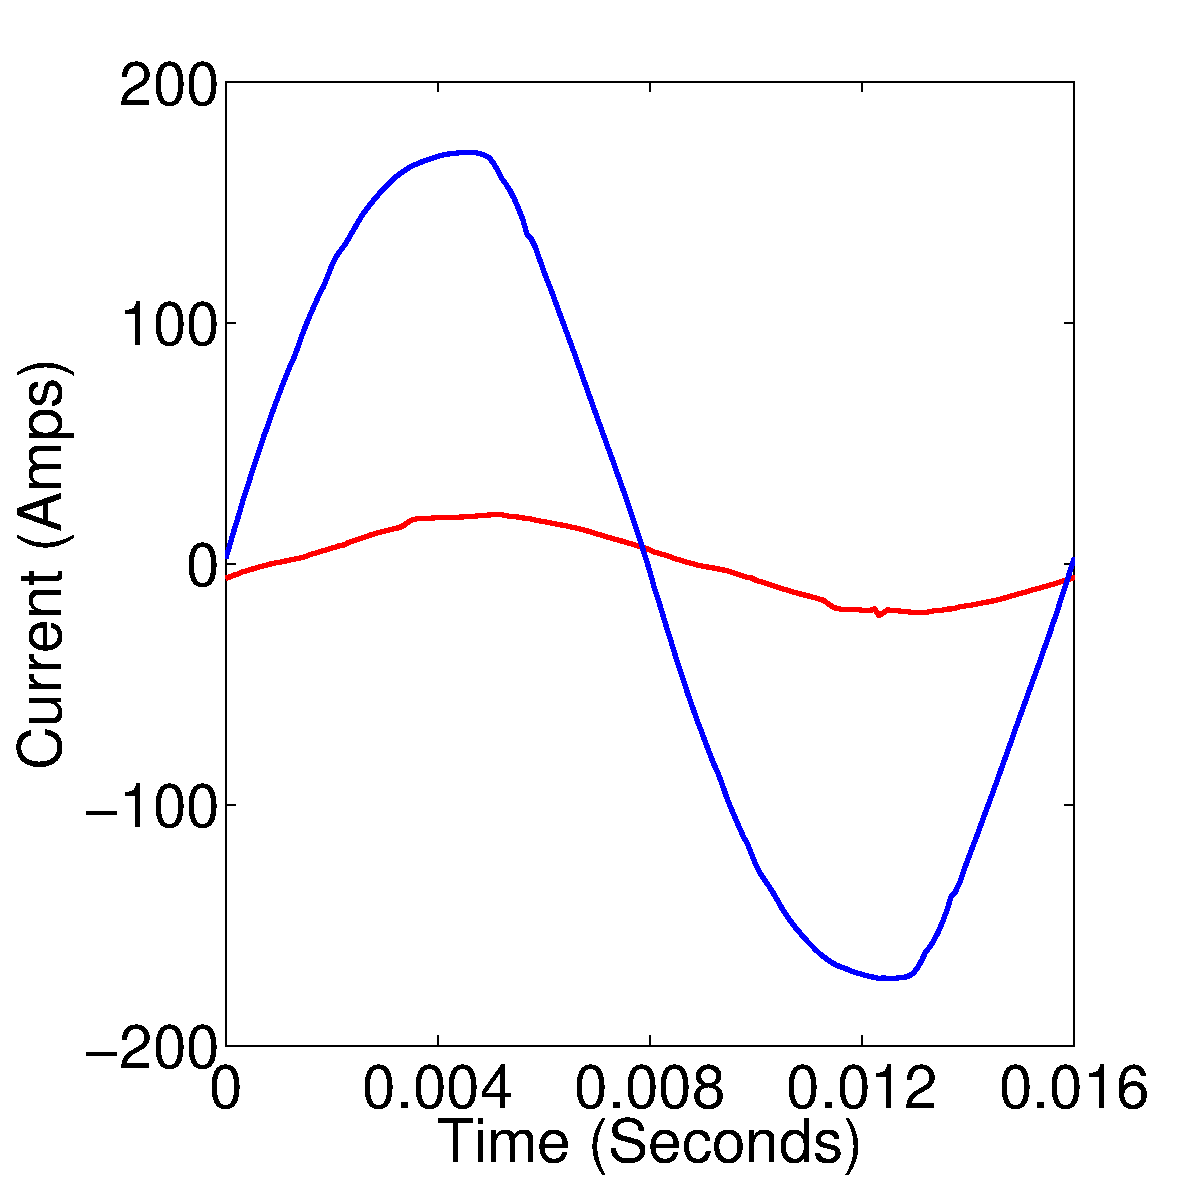
\includegraphics[width=0.3\textwidth]{figs/refrigeratorTransientCurrentVoltageSingle.pdf} \hspace{1em}&
	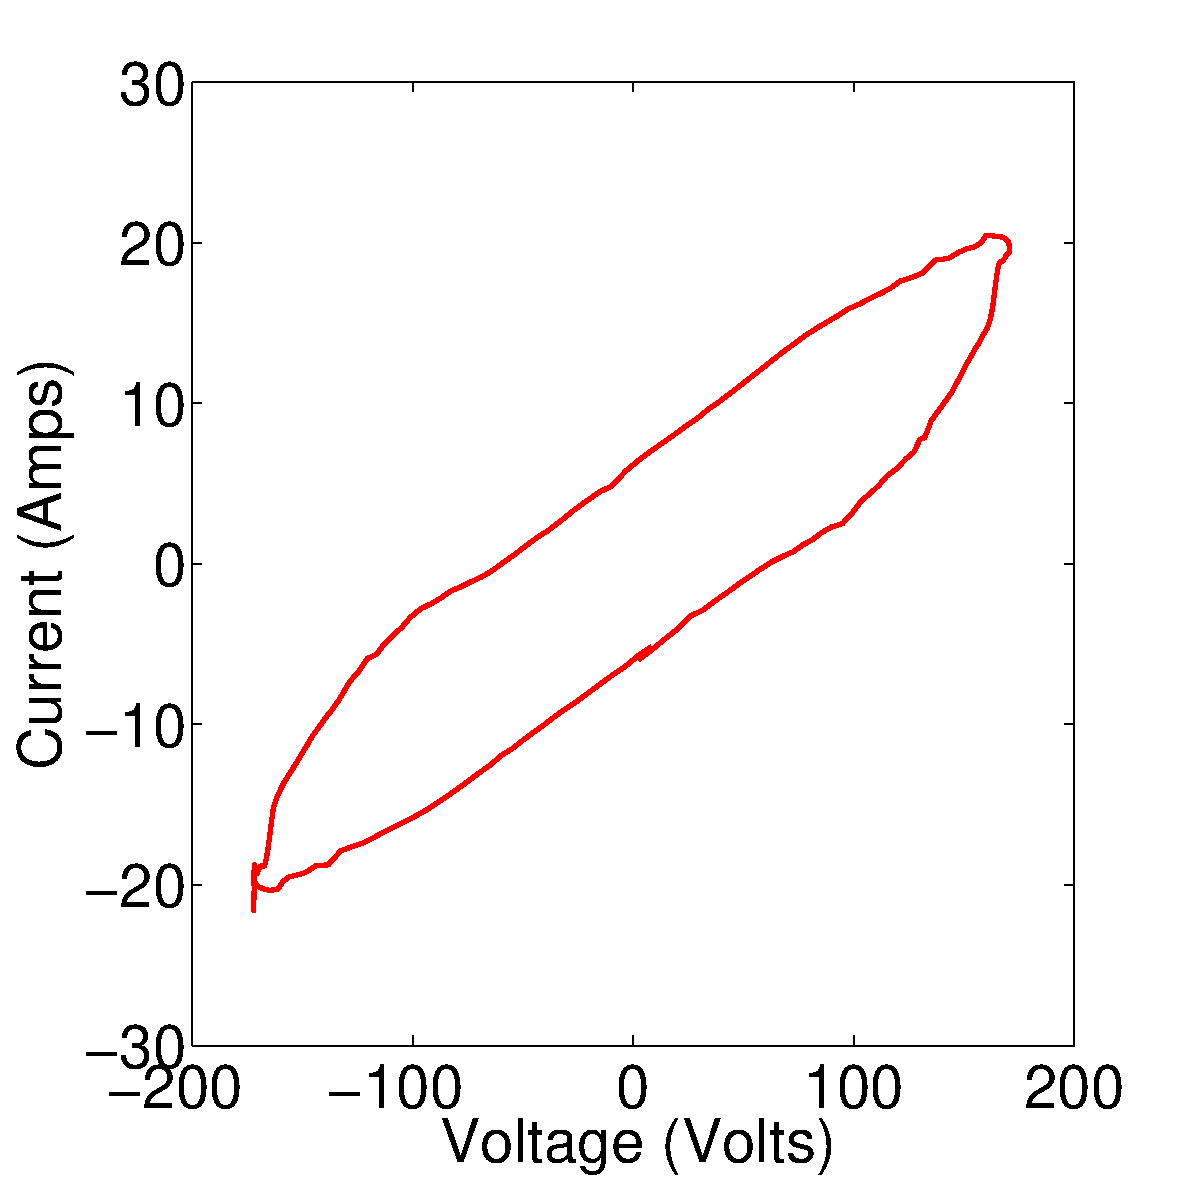
\includegraphics[width=0.3\textwidth]{figs/refrigeratorCurrentAgainstVoltageSingle.pdf} \tabularnewline

    (a) refrigerator & (c) refrigerator & (e) refrigerator \tabularnewline
        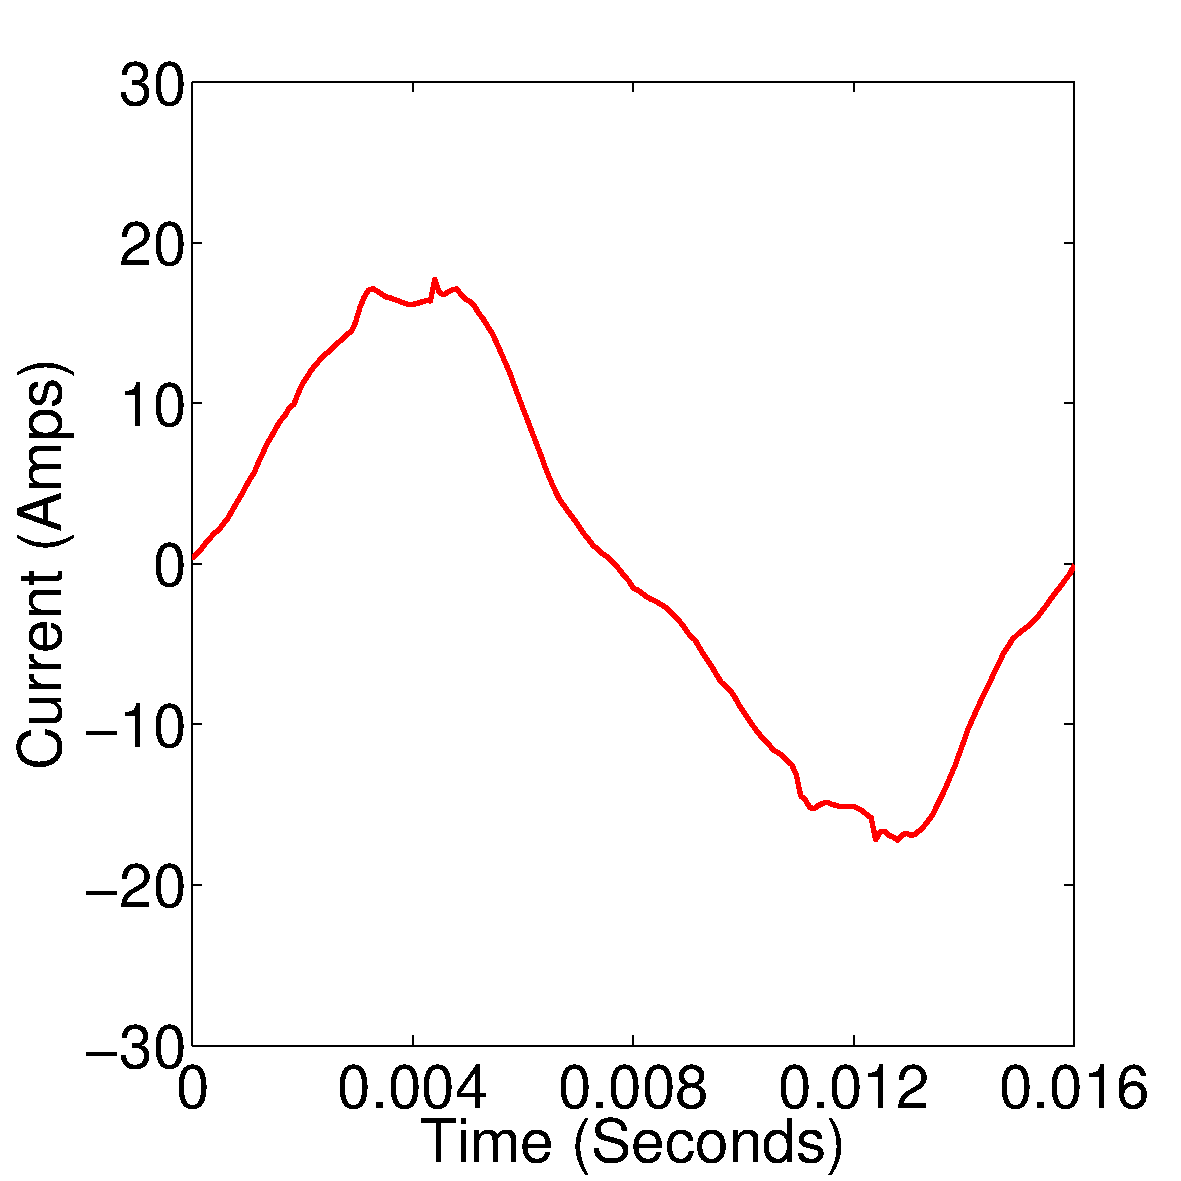
\includegraphics[width=0.3\textwidth]{figs/airCompressorTransientSingle.pdf} \hspace{1em}&	
        	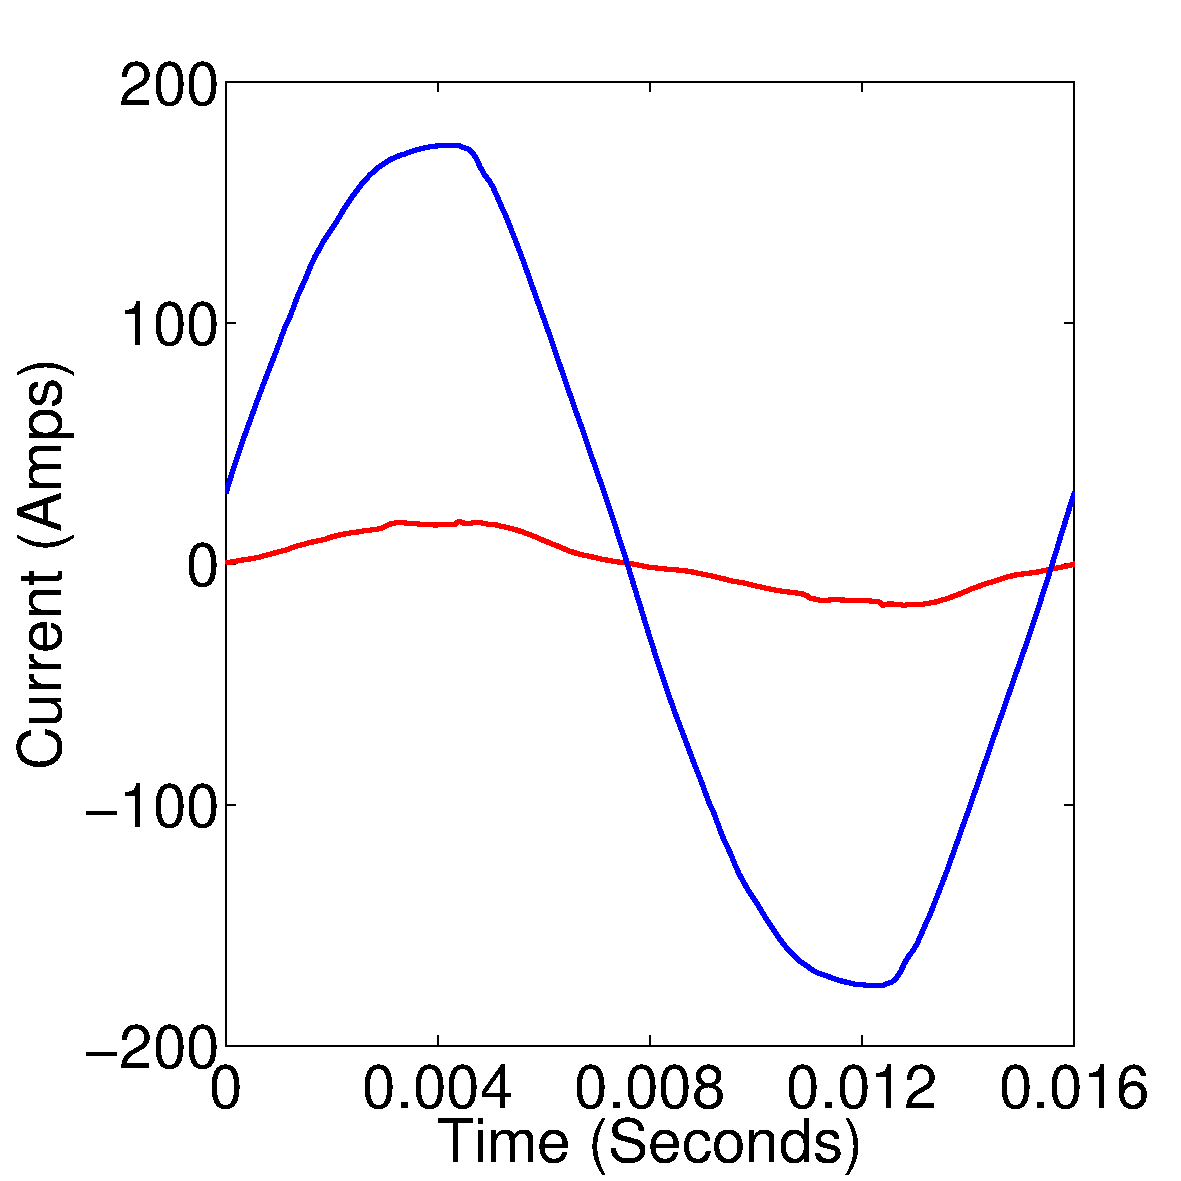
\includegraphics[width=0.3\textwidth]{figs/airCompressorTransientCurrentVoltageSingle.pdf}\hspace{1em}&	
	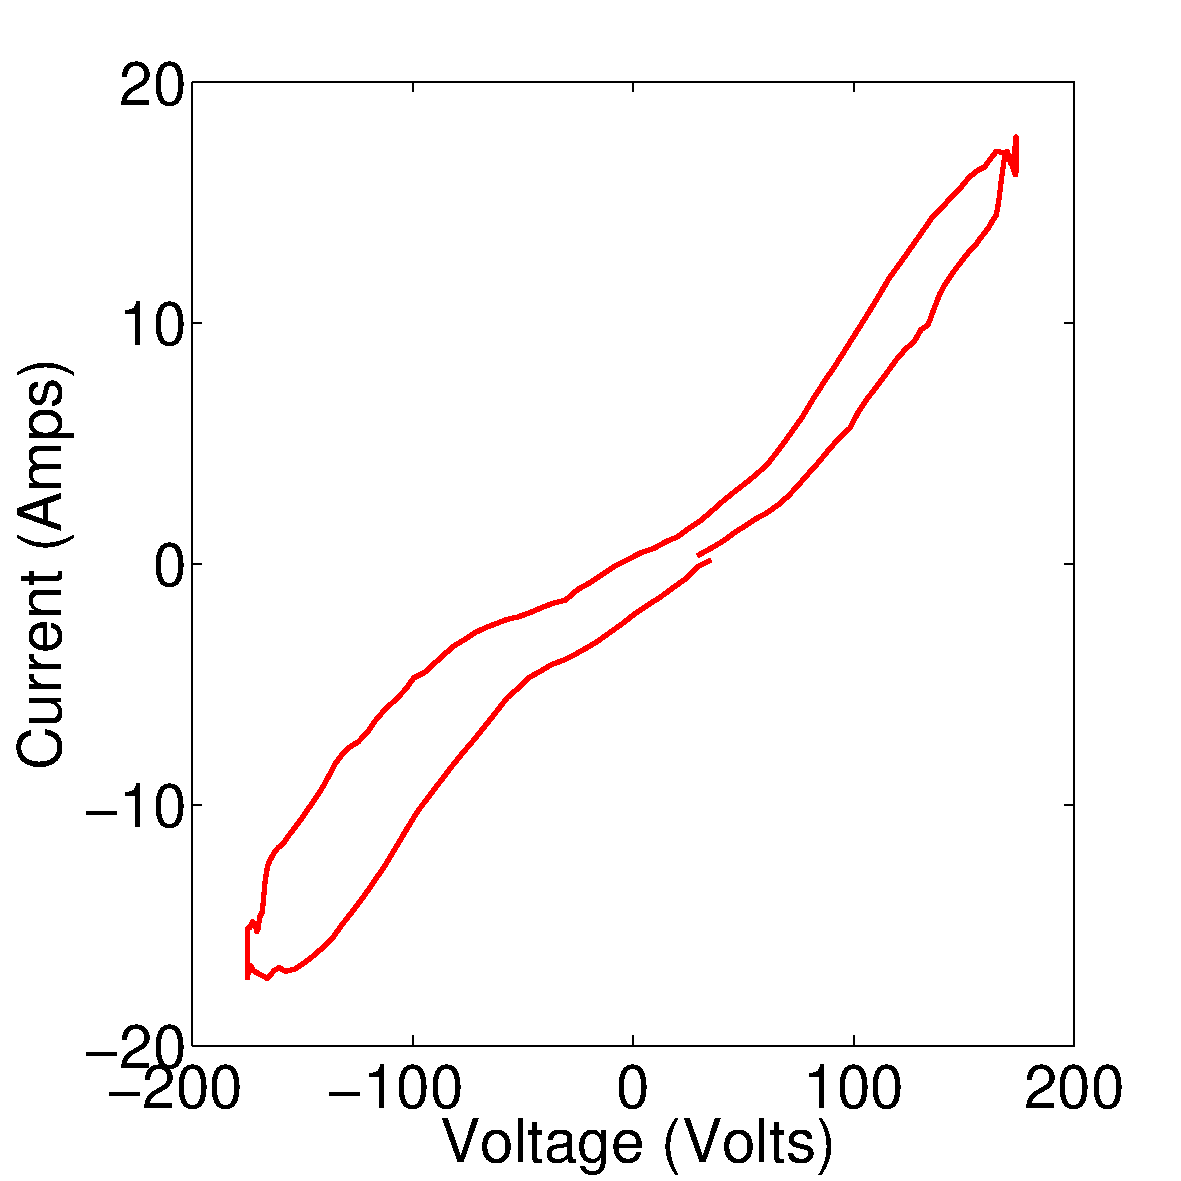
\includegraphics[width=0.3\textwidth]{figs/airCompressorCurrentAgainstVoltageSingle.pdf}\tabularnewline
    (b) air compressor & (d) air compressor & (f) air compressor \tabularnewline
    \end{tabular}
    }
	\caption{Current waveform of (a) a refrigerator and (b) an air compressor. The current and voltage of (c) a refrigerator and (c) an air compressor. The V-I trajectories of (e) a refrigerator and (f) an air compressor. }
	\label{fig_waveformTraj}
\end{figure*}
\cite{lam2007novel} utilize 
geometrical properties of V-I trajectories to sift between devices. 
\iffalse
\manishc{some of the figure refs seem to be off, can you verify? also, in fig
  13, (c) should be (d), and can you label the two rows of plots with 'refrigerator' and 'air compressor' 
}\huijuanc{add the label.}
\fi

Transformations of 
current or voltage waveforms, including the Fourier transform, 
 the wavelet transforms, 
and the eigenvalue decomposition are also useful. 
For instance, a short-time Fourier transform (STFT) approach has been used 
in~\cite{su2011feature} and 
\cite{chan2000harmonics} employs wavelet transforms of current 
or voltage waveforms 
to identify devices. 
%In the first stage, current or voltage waveform is transformed by wavelet transform.
%Then in the second stage, the wavelet characteristics of different devices
%are extracted and analyzed.
The eigenvalue of current or voltage waveforms is analyzed
as a feature in~\cite{liang2010load}. 
Figure~\ref{fig_eigenValue} depicts an example of how
two devices--- a circuit and dining room light---can be 
identified by eigenvalues.
These two devices both
have large first eigenvalues and small second eigenvalues. 
The difference between these two devices lie in that 
the first eigenvalue of the dining room light is larger than the first 
eigenvalue of the circuit. 
\begin{figure*}[h]
	\centering
	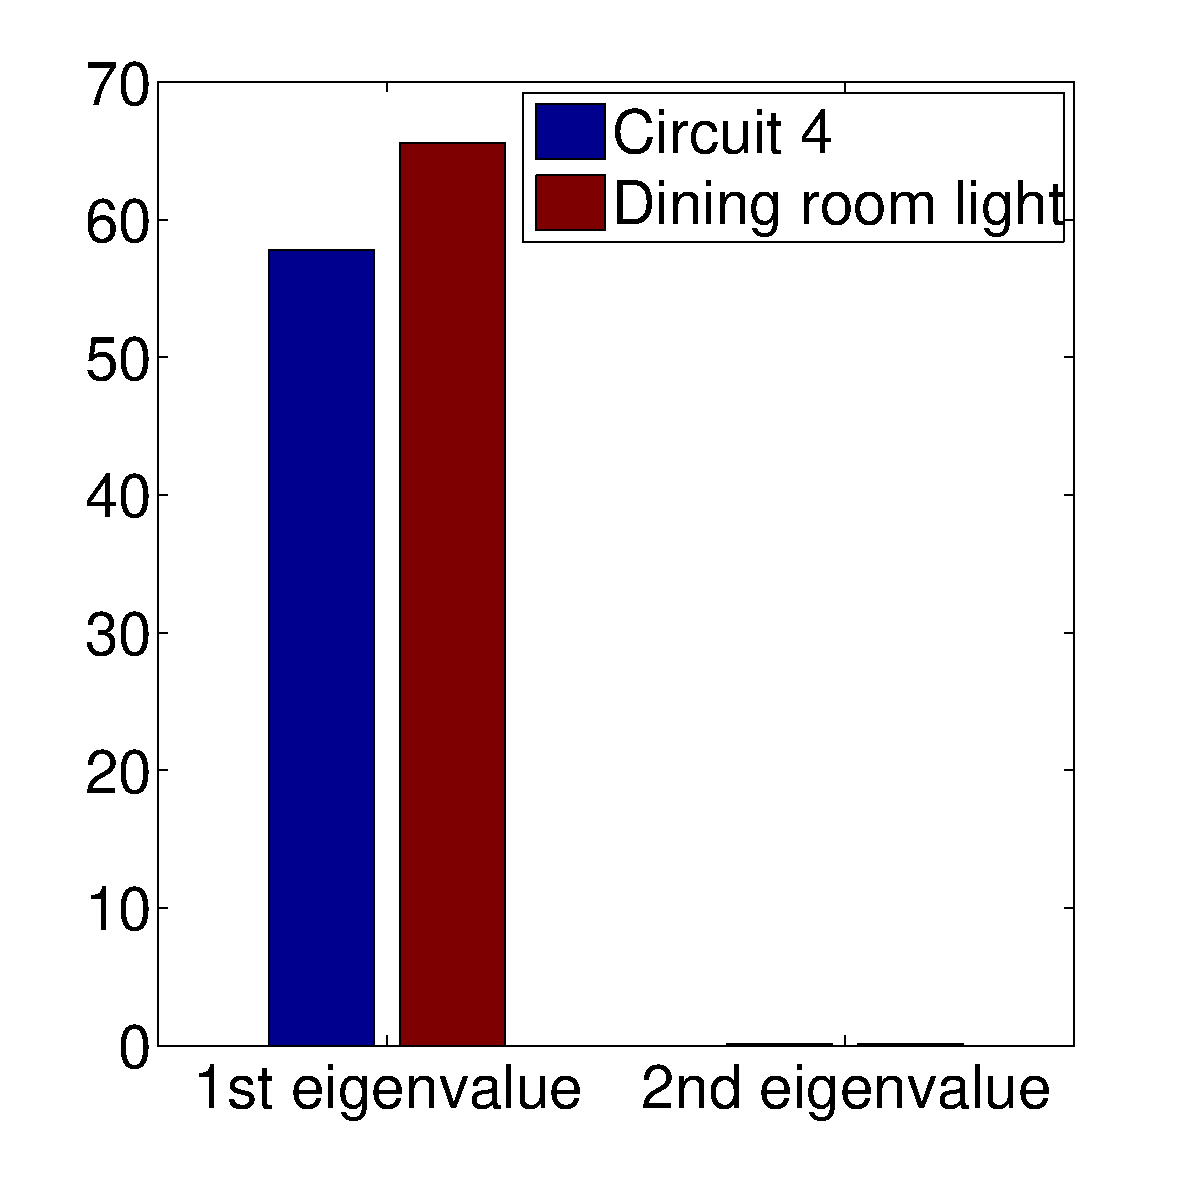
\includegraphics[width=0.3\textwidth]{figs/EigenValuesDevices.pdf}
	\caption{The eigenvalue of a circuit and dining room light. }
	\label{fig_eigenValue}
\end{figure*}


\textit{Harmonics:}
Harmonics constitute another class of features
defined over current or voltage waveforms.
Harmonics are integer multiples of the fundamental frequency of the waveforms. 
%\manishc{but what are harmonics? could you describe that in a senetnce or two?} \huijuanc{done.}
They are generated by non-linear devices such as VSDs,
electronic ballasts for fluorescent lighting,
switching power supplies, or rectifiers
when these devices start up or after they are on.
These waveforms are distorted to
be non-sinusoidal thus reflecting the inherent characteristics
of devices.
They play an important role in helping distinguish devices
when two devices share the same real power and reactive power. 
Harmonics can only be obtained from high frequency 
 data. 
%Equation (\ref{eq_harmonicsRange}).
%\begin{equation}
%\label{eq_harmonicsRange}
%f < N_{highest} \times 1/60 Hz
%\end{equation}

Figure~\ref{fig_harmonicsFeature} (a) and (b) illustrate the fact that, 
while an air compressor and refrigerator have similar real power,
by analyzing the first three harmonics
they can be distinguished.
Here, the magnitude of the first harmonic of air compressor is larger than 
that of the refrigerator. 
Also, the magnitude of the second harmonic of air compressor is smaller than 
the magnitude of the second harmonic of the refrigerator. 
\begin{figure*}[h]
\centering{
    \begin{tabular}{ccc}	
	
    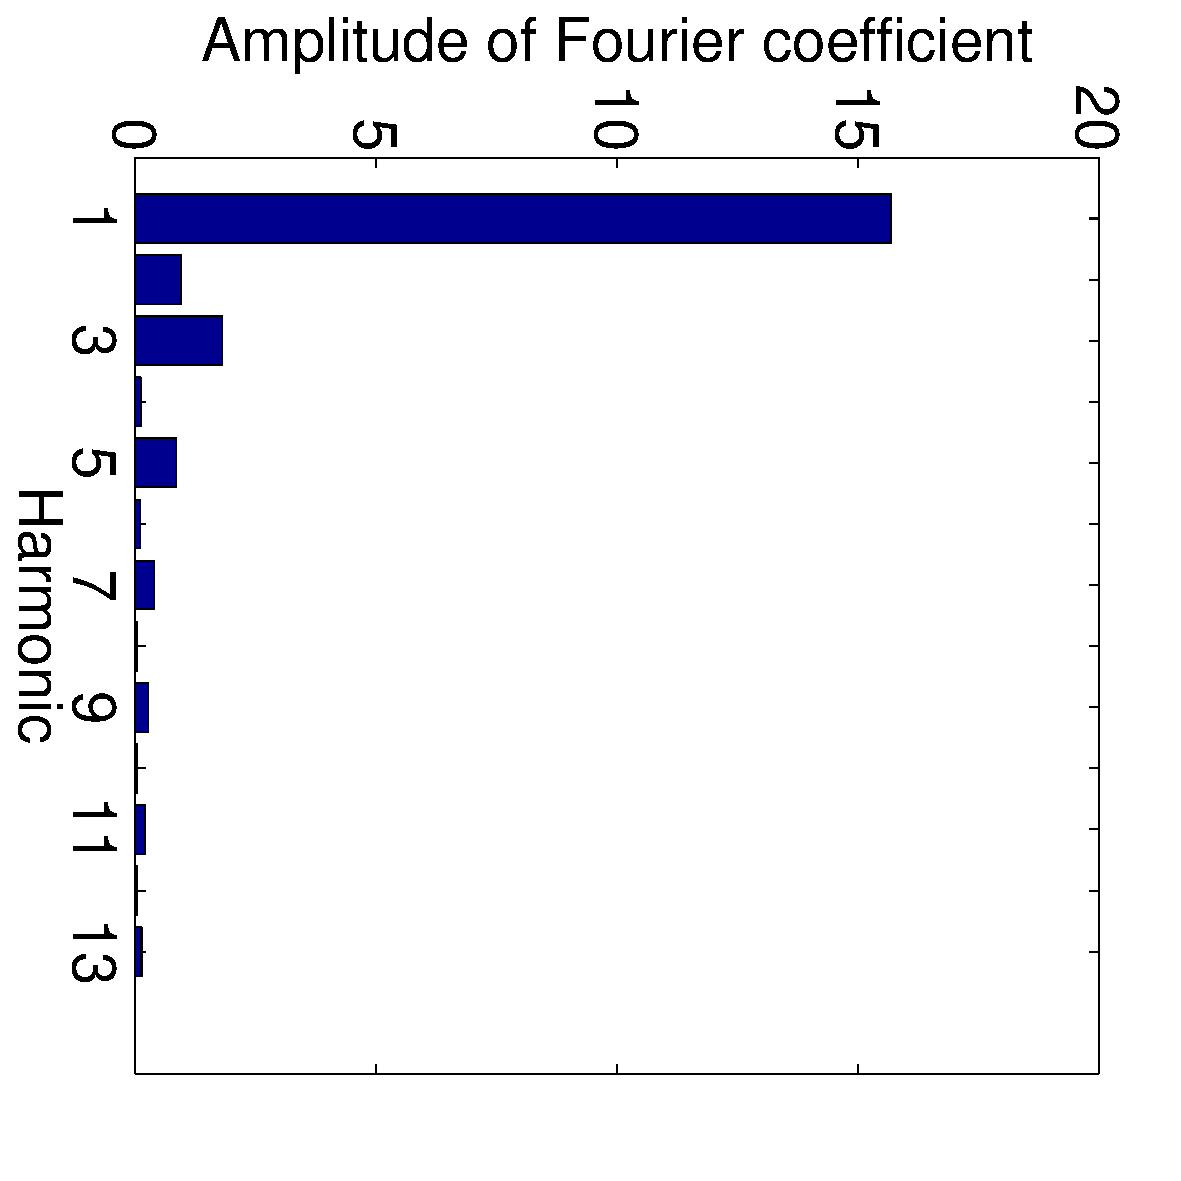
\includegraphics[width=0.33\textwidth,angle=90]{figs/refrigeratorTransientFFT.pdf} \hspace{1em}&
    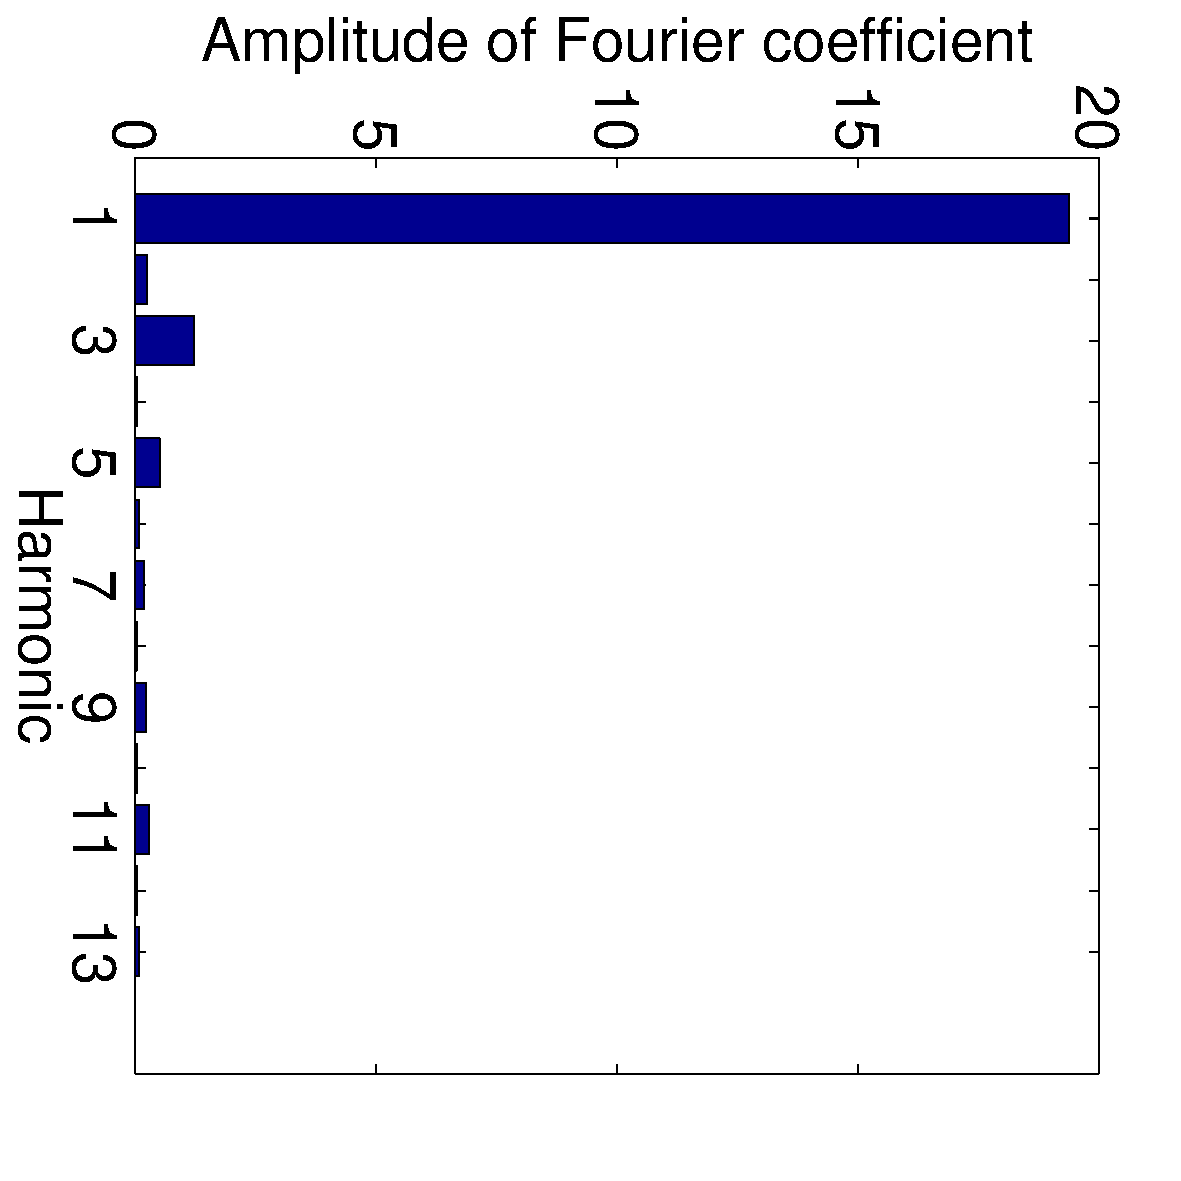
\includegraphics[width=0.33\textwidth,angle=90]{figs/airCompressorTransientFFT.pdf} \hspace{1em}&
    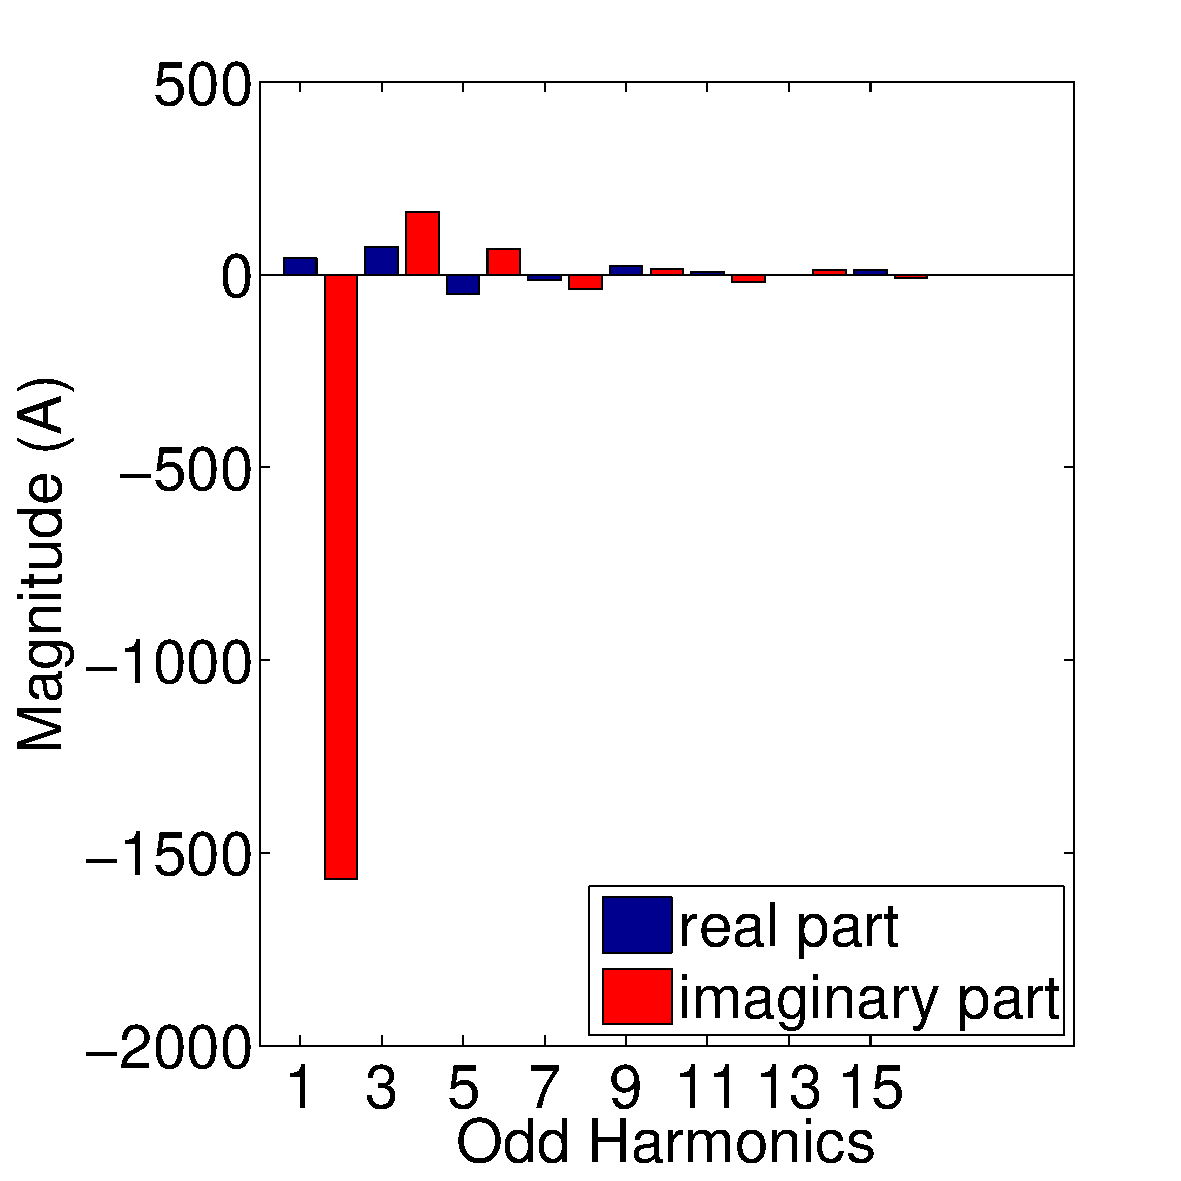
\includegraphics[width=0.33\textwidth]{figs/realImagHarmonicsRefrigerator.pdf} \tabularnewline
    (a) & (b) & (c) \tabularnewline
    \end{tabular}
    }
	\caption{Harmonics Feature of (a) a refrigerator and (b) an air compressor (c) real and imaginary part of odd number of harmonics of a refrigerator. }
	\label{fig_harmonicsFeature}
\end{figure*}


Harmonics have been employed in prior work 
\cite{laughman2003power,lee2005estimation,srinivasan2006neural,akbar2007modified,matthews2008auto,wichakool2009modeling}.
\iffalse
\huijuanc{will be deleted until huijuan's next comments.}
Some paper mentioned $N_{highest}$ as 11
because that's the highest useful harmonic for disaggregation.
\manishc{why?}.
Other papers~\cite{srinivasan2006neural} set $N$ to be 16 in order to capture more harmonics information
\manishc{but the previous senstence says that 11 is the highest useful harmonic}.
\huijuanc{change above sentences as follows.}
\fi
Generally only the odd harmonics are utilized. 
To the best of our knowledge, the highest employed harmonics are 
the 15 odd harmonics~\cite{srinivasan2006neural}. 
VSDs are hard to distinguish
but harmonics can be used to separate them. 
\iffalse
\huijuanc{delete until next comments of huijuan}
\cite{lee2003PhdThesis,lee2005estimation} thoroughly explained the approaches
as estimating the mean of higher harmonics of apparent power, 
then correlating the apparent power with the fundamental harmonic powers, 
thus identifying the VSDs \manishc{it is hard to understand this sentence,
  what is fundamental powers?  please re-word}
  \huijuanc{paraphrases as follows.}
 \fi
  \cite{lee2003PhdThesis,lee2005estimation} discovered that any VSD generates 
  a unique high harmonic power, which is identical among devices and effective for disaggregation. 
  Applying Gaussian random process to the power usage of VSD, 
  the $kth$ apparent harmonic power
  is calculated as $A_k=\sqrt{P_k^2+Q_k^2}$, where $k$ is the order number of 
the harmonics. 
The correlation pattern between the real power and 
the $kth$ apparent harmonic power is detected as a characteristic of each VSD. 

The real and imaginary parts of harmonics are also separately usable as features. 
Again, we only use the odd harmonics. 
The real part is calculated as 
$x_n=I_{(\frac{n+1}{2})}cos\theta_{(\frac{n+1}{2})}$ when $n$ is odd; 
%\manishc{how is the real part computed when n is even}\huijuanc{we only concern on the odd harmonics.}
the imaginary part is calculated as 
$x_n=I_{\frac{n}{2}}sin\theta_{\frac{n}{2}}$, 
for $n$ as even numbers, 
where $I_n$ is the magnitude of the $n$th current harmonic and
$\theta_n$ is the phase angle of the $n$th current harmonic. 
\iffalse
\manishc{are these equations only for odd harmonics? i vaguely remember that
  only odd harmonics are interesting. could you verify that, and find out why
  it is so, and include it here.}
  \huijuanc{Yes. That's the reason the paper of Srinivasan only mentioned the odd number of harmonics here.}
\fi
Figure~\ref{fig_harmonicsFeature} (c) shows the real part and imaginary part 
of the odd harmonics of a refrigerator. 
Also,~\cite{srinivasan2006neural} gives an example of how to separate devices 
by the real and imaginary part of harmonics. 

A variant of harmonics is the spectral envelope. 
This is a short-time average of harmonics 
and was proposed as a device feature in~\cite{leeb1995transient,laughman2003power}.
Further, harmonics can be used in conjunction with other features to disaggregate devices. 
\cite{wichakool2009modeling} introduces a switching-function 
to identify variable speed devices. 
\iffalse
\manishc{you use VSD in a lot of places,
  could you use the full expansion when it is used the first time, and then
  use VSD}\huijuanc{VSD has been explained in page 5. Is it necessary for us to list 
  all the abbreviations before the introduction section?}. 
\fi  
\begin{figure}[h]
\centering
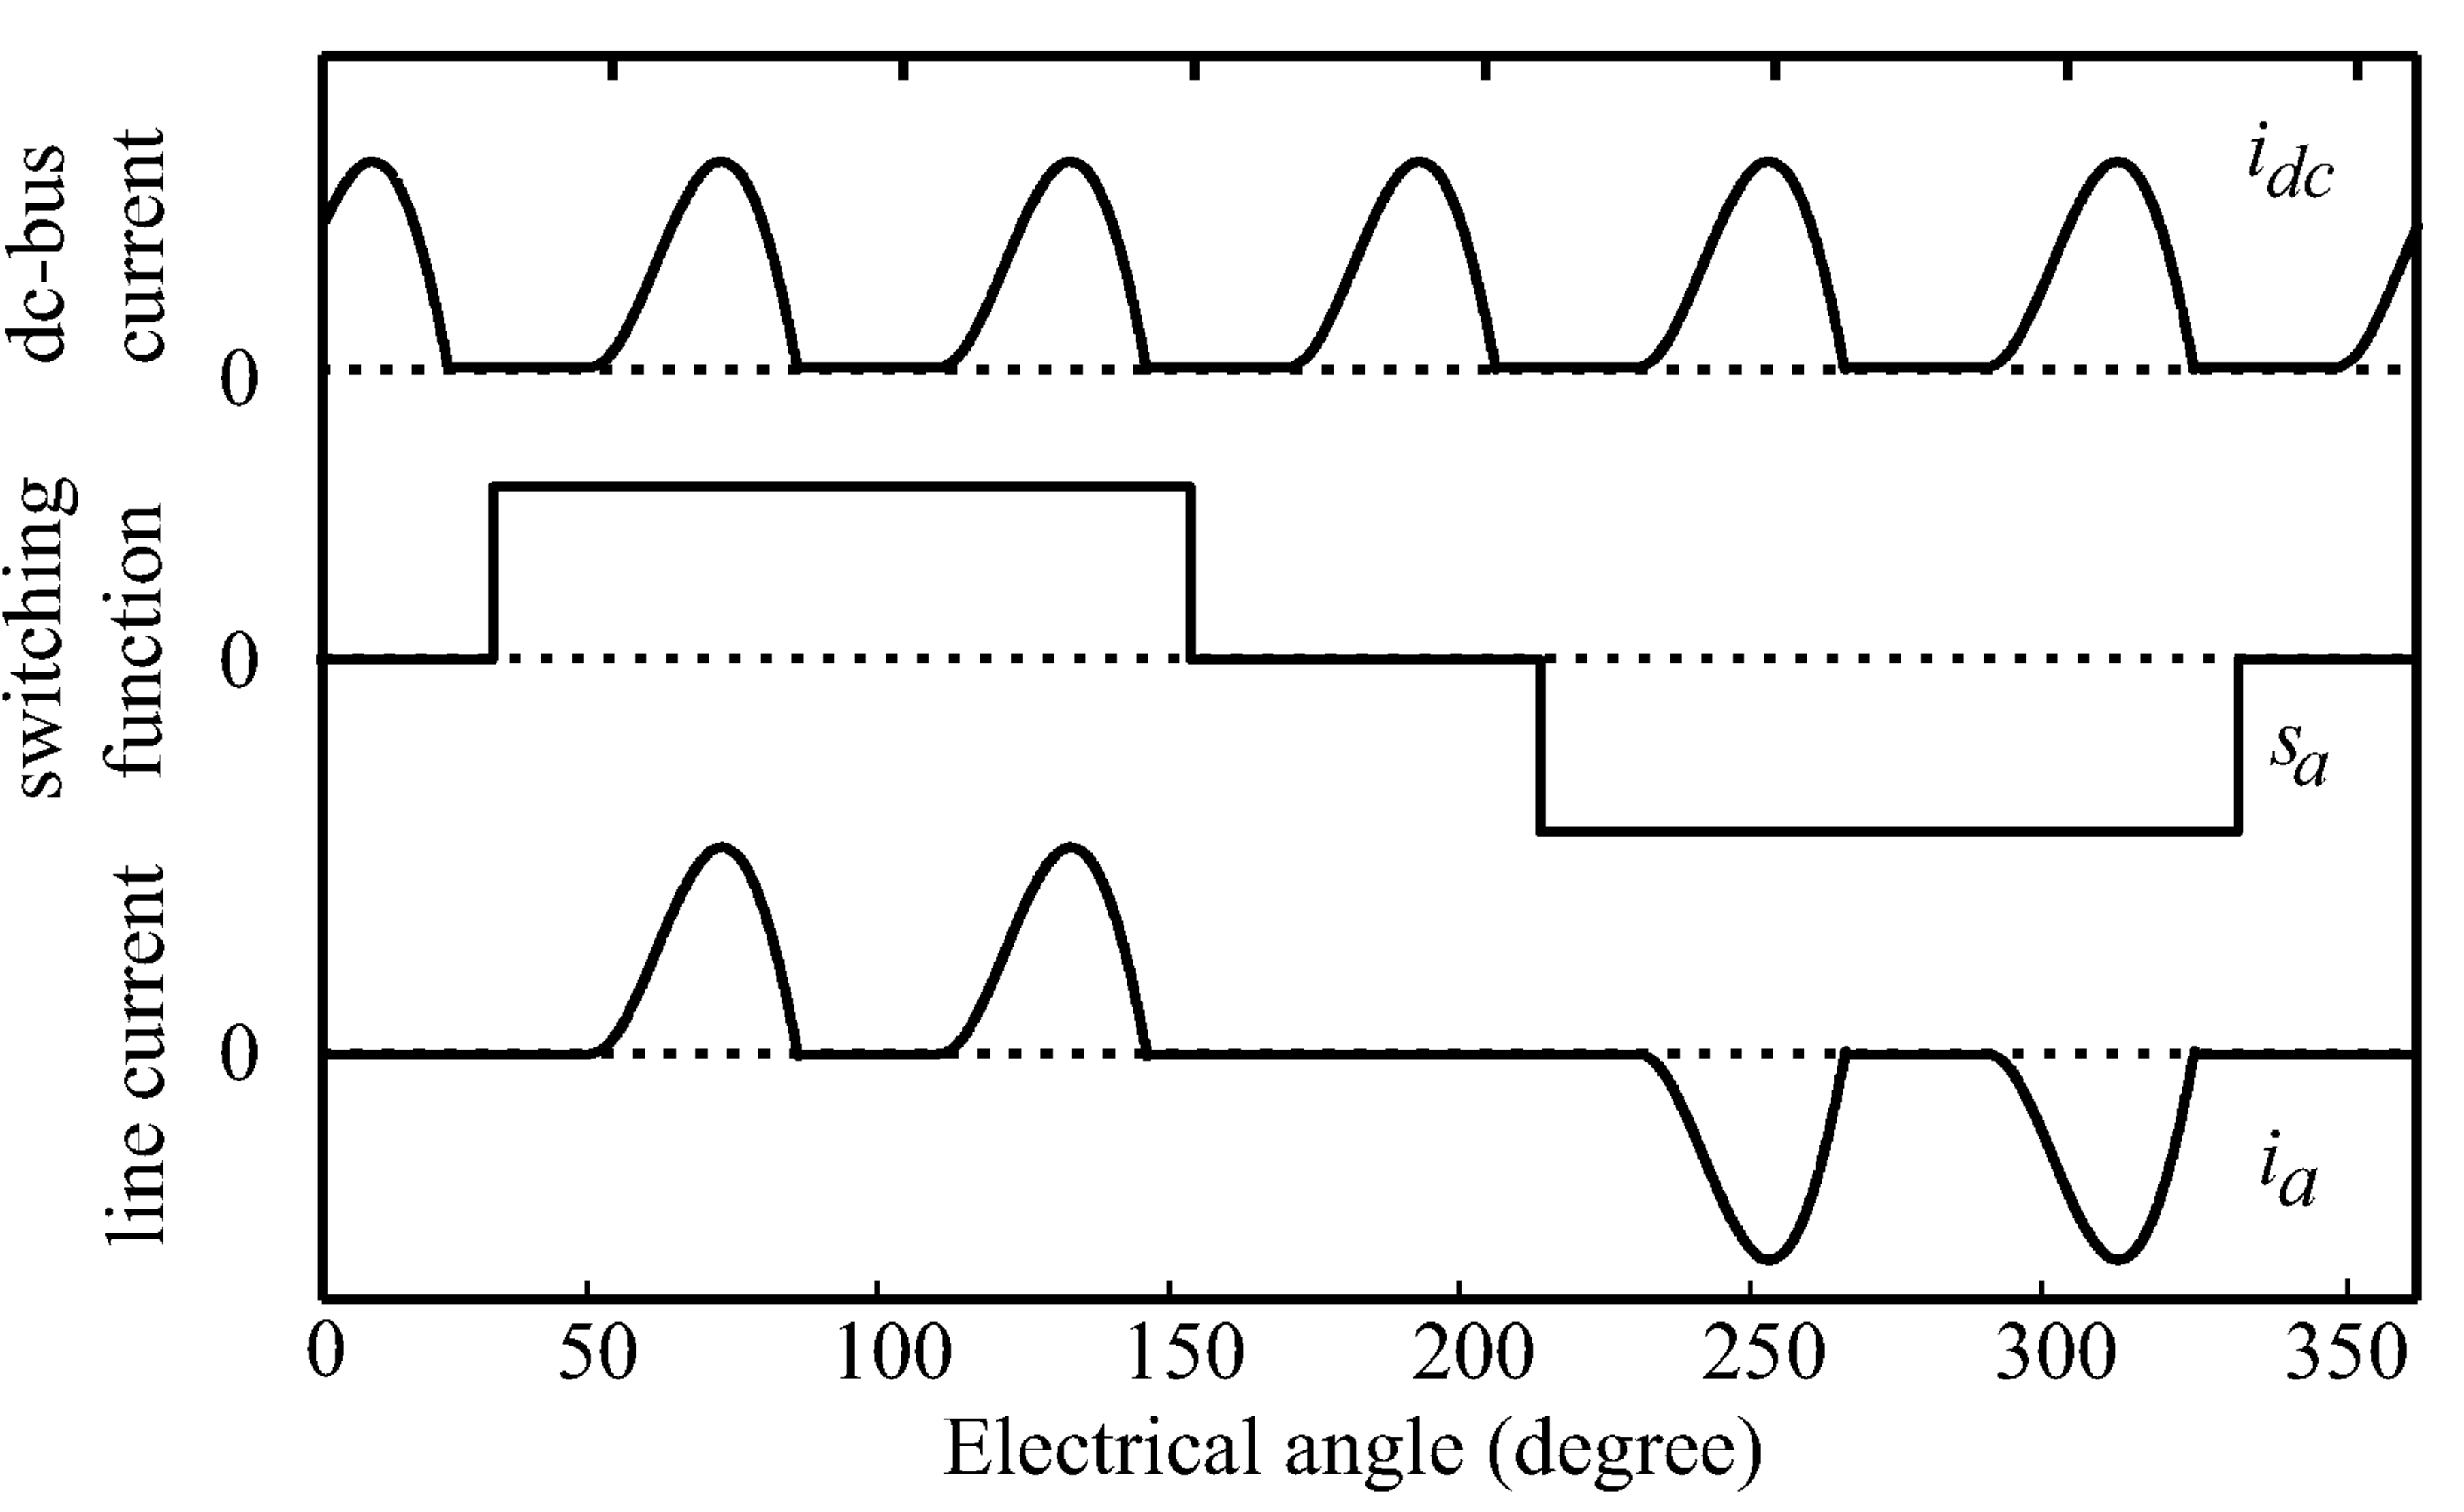
\includegraphics[width=0.5\textwidth]{figs/switchingFunction.png}
\caption{Switching-function for VSDs disaggregation (Courtesy:\cite{wichakool2009modeling}).}
\label{fig_switchingfun}
\end{figure}

Figure~\ref{fig_switchingfun} gives a comparison example
of current before and after rectifier and inverter of VSDs.
The operations of the rectifier of a VSD correspond to
a switching function.
The current is initially direct current $I_{dc}$ and
after the current goes through the switching process,
it changes to $I_a$.
The relationship between these two currents
is captured as $I_a(\theta)=S_a(\theta)I_{dc}(\theta)$, 
where $S_a(\theta)$ is the switching function. 
This switching function can be represented as 
a linear combination of different harmonics: 
$S_a(\theta)=S_0+\sum_n(S_n^p \sin n\theta - S_n^q \cos n\theta)$, 
where $n$ is the harmonic number, $S_0$ is the DC component,
and the variables $S_n^p$ and $S_n^q$ are the magnitudes of
the in-phase and quadrature parts of $nth$ harmonics of the
switching function. 
By comparing the Fourier coefficients with the $S_n^p$ and $S_n^q$ of harmonic coefficients,
these VSDs can be recognized.

\textit{Noise data:}
\cite{patel2007flick} and~\cite{gupta2010electrisense} recorded 
noise data instead of the current or voltage data.
Interestingly, this noise data
which occurs during switching on or off, 
can be used to identify devices
because different devices have different noise signatures. 
The frequency of the noise data is also treated as a feature. 
\cite{patel2007flick} first detects that noise is generated 
when a device in a residential building
turns on or off, or during the on state. 
With the introduction of switch mode power supplies (SMPS), 
the EMI generated by SMPS has also been
considered
as a feature~\cite{gupta2010electrisense}.
Figure~\ref{fig_LCDTVNoise} (a) depicts
the frequency generated by an LCD TV's on and
off events from
the Kaggle dataset~\cite{kaggle2013energy}.
Figure~\ref{fig_LCDTVNoise} (a) illustrates the noise time series background in red and 
the noise time series with newly added noise in blue. 
Figure~\ref{fig_LCDTVNoise} (b) shows that the newly added noise is segmented. 
By analyzing the mean value and standard deviation of the segmented noise, 
SMPS devices can be identified. 
\begin{figure}[ht]
\centering{
    \begin{tabular}{cc}	
	
    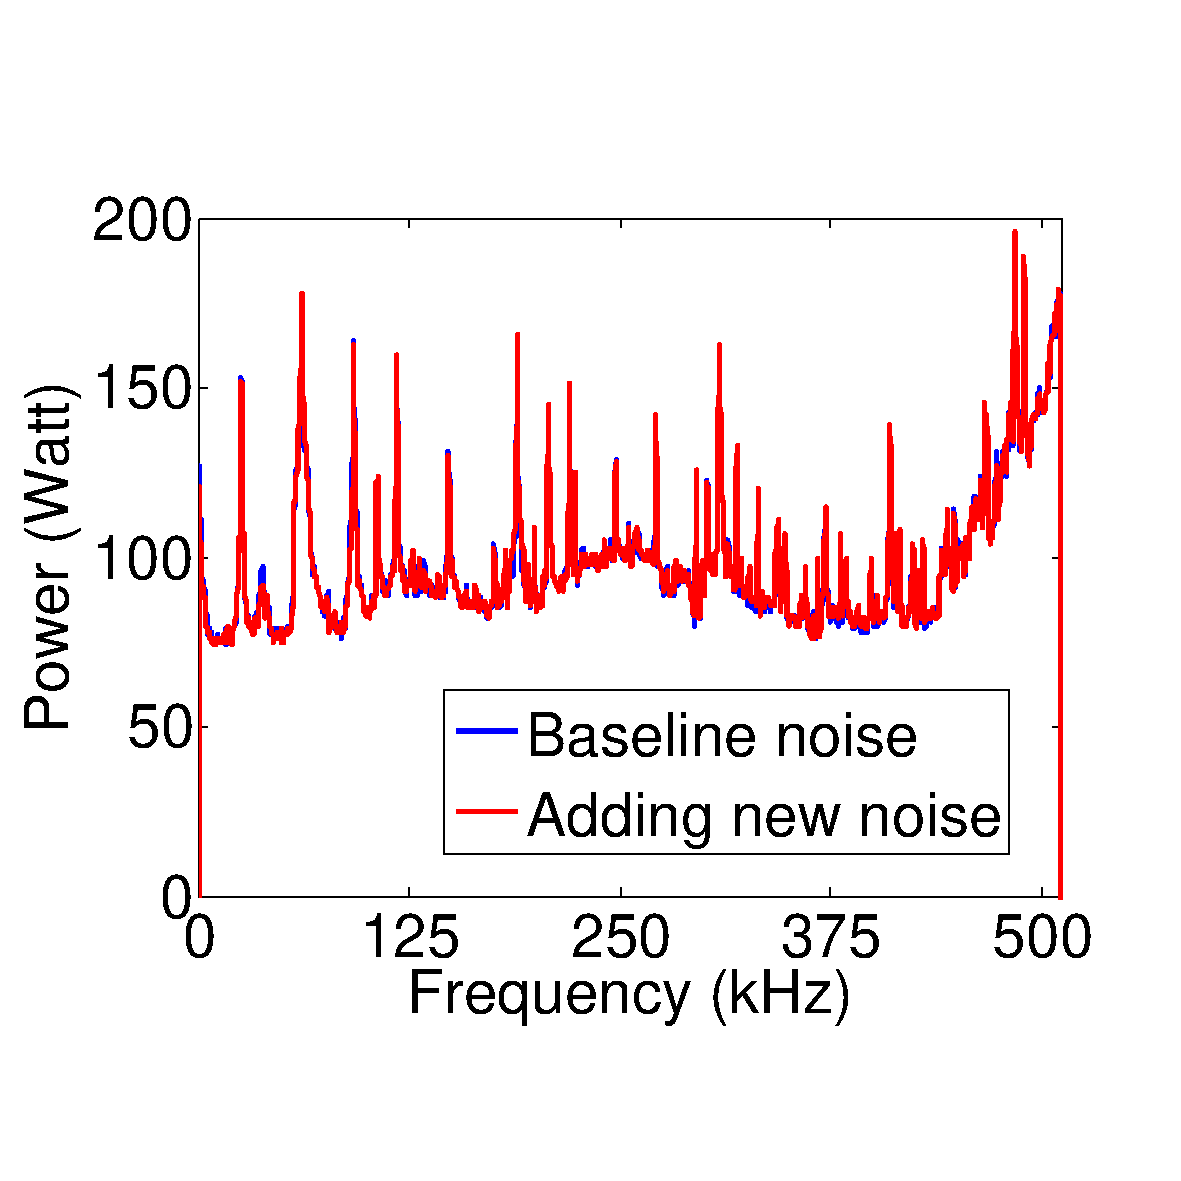
\includegraphics[width=0.5\textwidth]{figs/noiseMasterLCDTV.pdf} \hspace{1em}&
   % 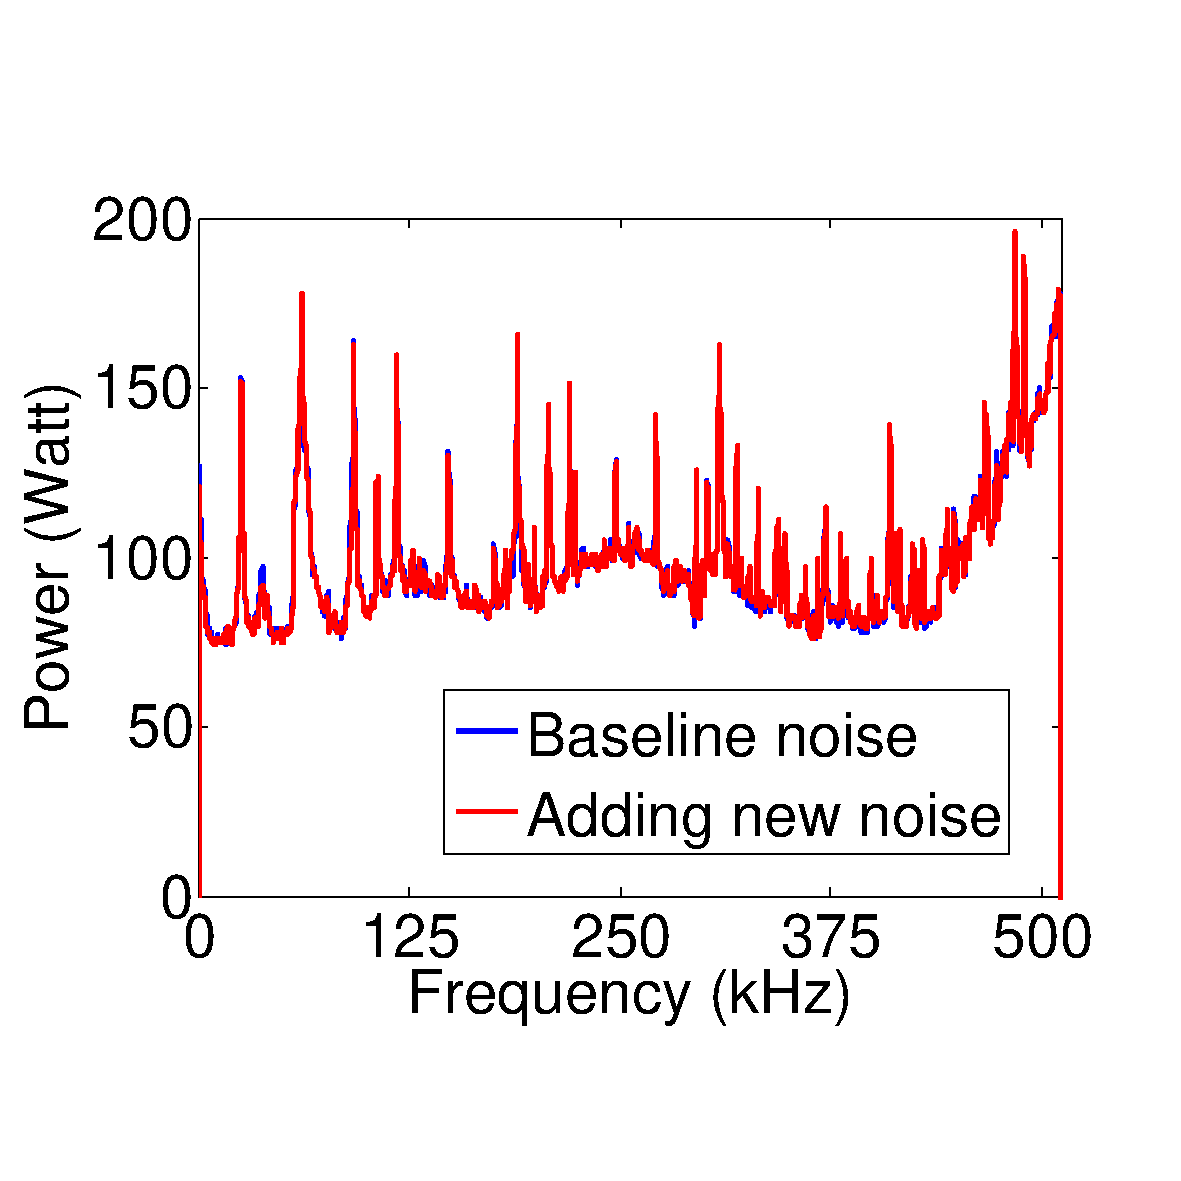
\includegraphics[width=0.3\textwidth,height=0.23\textheight]{figs/noiseMasterLCDTV.pdf} \hspace{1em}&
    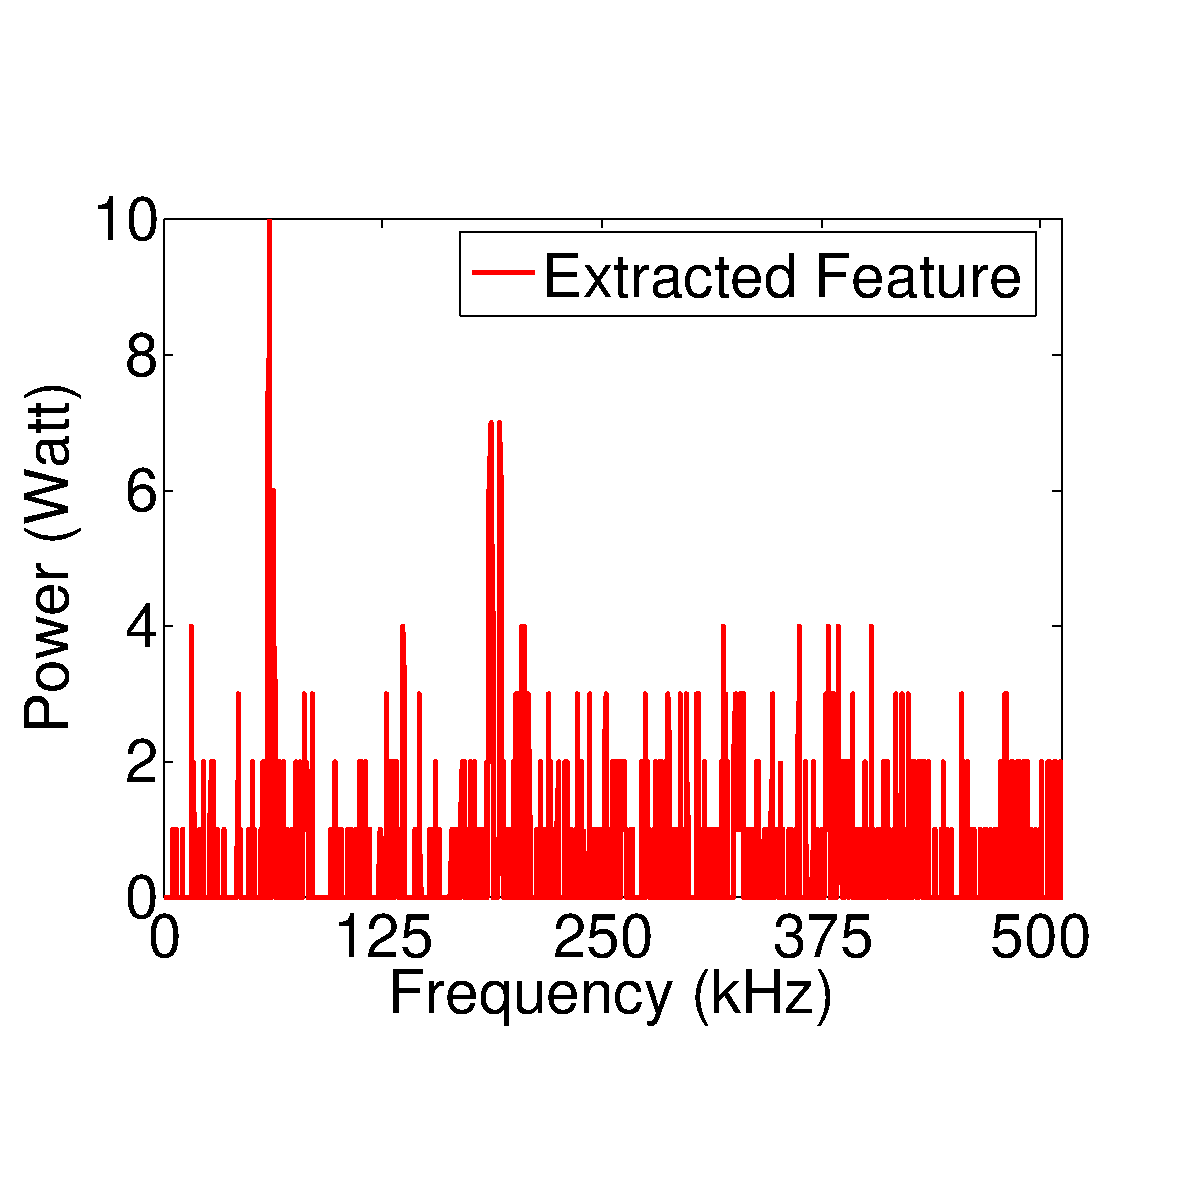
\includegraphics[width=0.5\textwidth]{figs/noiseFeatureMasterLCDTV.pdf} \tabularnewline
    (a) &(b) \tabularnewline 
    \end{tabular}
    }
\caption{(a) Baseline noise with newly added noise. (b) Noise Feature of a device.}
\label{fig_LCDTVNoise}
\end{figure}
 

%\manishc{can you increase the font size of the text in fig 17, it is hard to read}\huijuanc{done.}

\subsection{Features beyond Current and Voltage}
%Besides AC-power values related to current and voltage,
%there are also additional features,
%such as time features,
%correlation between devices,
%electromagnetic field (EMF) emitted by devices,
%and etc.

\textit{Duration or time of use}
The operation of a device may conform to
a routine schedule of
when it is turned on or off,
and how long it is on or off.
The time of device usage involves the
month of the year, day of the month, day of week, time of the day,
and season of the year.
Generally, fans and air-conditioners
work in the summer and heaters work in the winter.
Figure~\ref{fig_timeofday} shows 
the total power usage of a commercial building~\cite{shao2013temporal}.
%\manishc{fig 18 caption should read 'day of week ...'}\huijuanc{done.}
Power usage is high during a weekday. 
In contrast, the power usage on weekends is quite low. 
\begin{figure*}[h]
	\centering{
    \begin{tabular}{c}	
	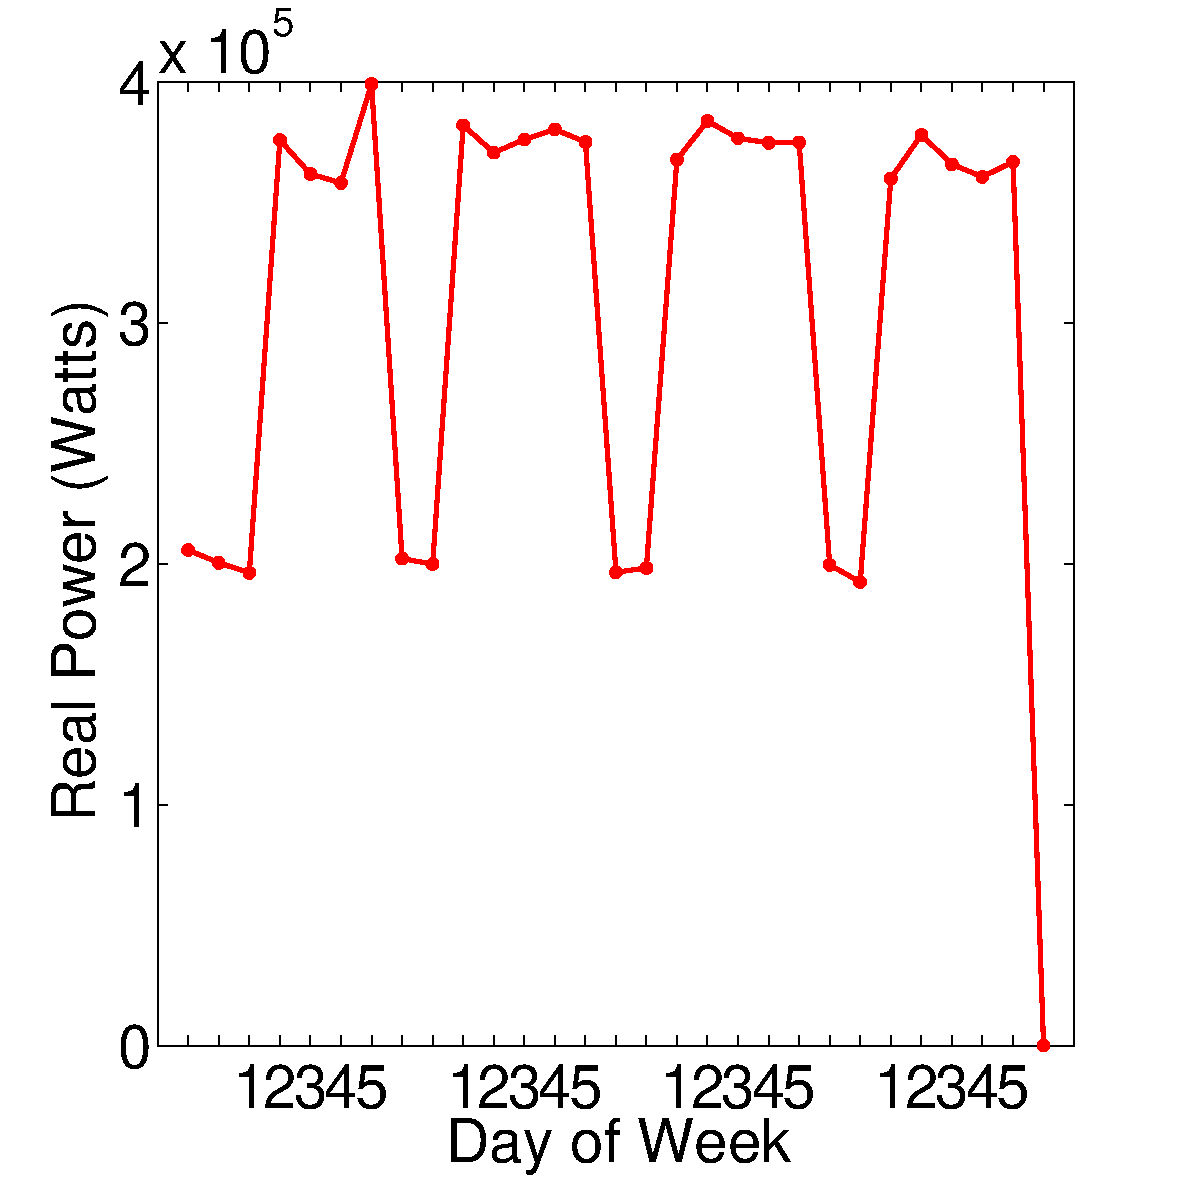
\includegraphics[width=0.3\textwidth]{figs/timeofday.pdf}
	%\includegraphics[width=0.3\textwidth,height=0.3\textheight]{figs/onduration_kim2010unsupervised.png} \hspace{1em}&
%    \includegraphics[width=0.5\textwidth]{figs/coefficients_kim2010unsupervised.png} \tabularnewline
   % (a) & (b) \tabularnewline
    \end{tabular}
    }
	\caption{Day of Week of Feature.}
	\label{fig_timeofday}
\end{figure*}


Date, time, and week features have been used in previous work.
For example,~\cite{kim2011unsupervised} points out that
a laptop is often powered-on in the morning of workdays
and that the TV is powered on during the evenings and weekends. 
Also,~\cite{kim2011unsupervised} analyze the on/off
distribution of devices and find that
they conform to a Gamma distribution.

\textit{Device correlation}
Some devices may need to operate with other devices.
For example, the TV and Xbox usually turn on and off
together.
Such correlation between devices has been
analyzed and integrated with a HMM-based model~\cite{kim2011unsupervised}.
This study calculates all the correlation coefficients and 
shows that 
both the correlation between TV and stereo
and the correlation between XBox and TV were as strong as 0.8.
\cite{chen2013novel} combines the features of on/off time, duration, and the correlations 
among devices to mine for usage patterns. This approach is 
designed especially for 
correlations between different 
types of devices other than the devices of the same type. 
In continuing work,~\cite{chen2014mining} develop an algorithm (CoMiner) to discover 
correlation between devices. 

\textit{EMF, sound, and light.}
Electromagnetic fields (EMFs)
are generated by electrical devices
when they are powered on.
Different devices can result in different EMFs which
can be monitored by an EMF sensor around devices.
This idea is used in~\cite{giri_study_2012}
to detect on/off state changes of devices.
In addition, sound and light resulting from
devices can help judge the status
of devices as described in~\cite{kim2009viridiscope}.
This work monitors sound by an acoustic sensor 
at 4Hz sampling rate
to identify the compressor status of a refrigerator. 
Also, the light intensity from a sensor installed in a refrigerator reflects 
whether the door is open or closed.

%%delete too long, unnecessary
%Figure\ref{fig_soundLightFeature} (a) 
%illustrates how sound measured by an acoustic sensor 
%identifies the compressor status of a refrigerator. 
%It shows that an acoustic sensor at 4 Hz sampling rate can detect the
%on/off status of the compressor.
%Figure\ref{fig_soundLightFeature} (b) 
%depicts the case that a light inside 
%a refrigerator monitors whether the 
%door opens or shuts. 
%It shows that light intensity in a refrigerator goes up when the door is
%open and the inside light is on.
%\begin{figure*}[ht]
	\centering{
    \begin{tabular}{cc}	
	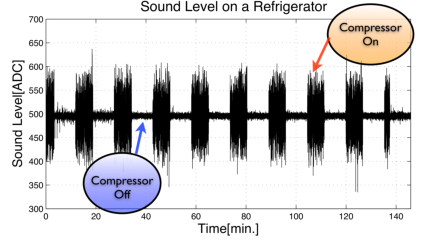
\includegraphics[width=0.5\textwidth]{figs/kim2009viridiscope_sound.pdf} \hspace{1em}&
    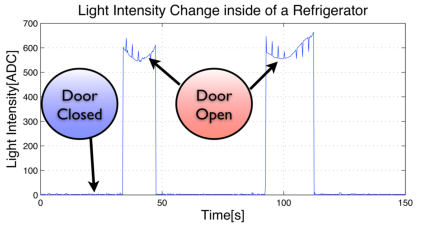
\includegraphics[width=0.5\textwidth]{figs/kim2009viridiscope_light.pdf} \tabularnewline
    (a) & (b) \tabularnewline
    \end{tabular}
    }
	\caption{(a) compressor detection by acoustic sensor and (b) refrigerator detection by light. (courtesy: \cite{kim2009viridiscope}).}
	\label{fig_soundLightFeature}
\end{figure*}



\textit{Weather.}
Weather is a key factor for a commercial building's power usage
because of variation in the usage of the HVAC system in the summer and winter.
The correlation between temperature and electricity usage 
is studied in~\cite{pardo2002temperature}. 
%Figure \ref{fig_pardo2002temperature_temp} shows that, 
This work exploits the fact that
when the temperature is higher, 
the daily electricity usage increases. 
%\begin{figure}[ht]
%\centering
%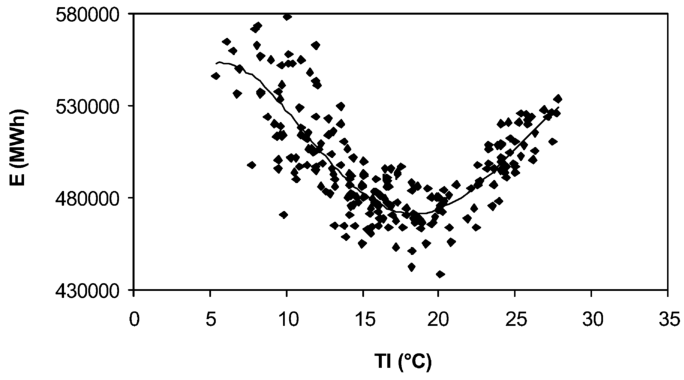
\includegraphics[width=3 in]{figs/pardo2002temperature_temp.pdf}
%\caption{Variation of the total daily electricity load in Spain with the temperature index in 1998
%(courtesy: \cite{pardo2002temperature}).}
%\label{fig_pardo2002temperature_temp}
%\end{figure}

\textit{Other possible features.}
Additional sensors, such as motion sensors~\cite{cook2011sensor}, 
can determine activity inside a building, and provide useful input to a
disaggregation model.
\cite{srinivasan2013fixturefinder} integrates data from electricity 
and other sensors at home to disaggregate  low-power 
devices such as lightbulbs. \cite{wu2012low} proposes using plug-in low-cost outlet sensors to help capture 
appliance state. 
Also, ~\cite{uttama2013sustainable} uses limited plug-level sensors to improve 
disaggregation accuracy. 
In the future, more sensors are likely to be available and could be leveraged for 
energy disaggregation.

%Other factors like price may play a role.
%When the electricity price increases,
%people resort to other energy instead of electricity.

%idea: to be used in future research, not mention it in this paper?

%Low frequency data means the current/voltage
%waveform cannot be recovered by the sampling data.
%High frequency data refers to those data
%from which the current or voltage can be reconstructed.
%%and can be obtained from both
%low frequency and high frequency recorded data.
%However normally reactive is Not logged by reactive
%power meter because the cost of
%reactive power meter is high thus not used in
%energy disaggregation.
%Even though, reactive power and power factor
%can still be calculated by calculating the
%voltage and current values from the high
%frequency data, which can recover the
%voltage and current waveform.


%%%%%%%%%%%%
%For any circuit, we can classify the current and
%voltage response as the sum of a transient response
%and a steady response.
%For any voltage or current as a function of time,
%it can be written in form of
%\begin{equation}
%x(t)= x_T(t)+x_{SS}
%\end{equation}
%page 192 in book \cite{courtesy: eebook1}
%where $x(t)$ can represent both current and voltage.
%$x_{T}(t)$ is the transient state and
%$x_{T}(t)=(x_0-\tau F)e^{-\frac{t}{\tau}}$.
%$x_{SS}$ denotes the steady state.
%%%%%%%%%%%%%%%%%%%%%

